\documentclass[
    parspace,
    noindent,
    nohyp,
    %final, % hide todos
]{elteiktdk}[2023/04/10]

\usepackage[dvipsnames]{xcolor}
\usepackage{graphicx}
\usepackage{colortbl}
\usepackage{svg}
\usepackage{float}
\usepackage{pgfplots}
\usepackage{arydshln}
\usepackage{fontawesome}
\usepackage{picture,xcolor}
\usepackage{fancyvrb}

\newcommand{\rhpad}{\vspace{0.6\baselineskip}}

\newcommand{\thesispar}[1]{
\vspace{1em}
\hspace{0.7cm}\parbox[left][][c]{15.8cm}{\linespread{1.2}\selectfont #1}
\vspace{1em}
}

\usepackage[newfloat]{minted}
\AtBeginEnvironment{minted}{\singlespacing}

\title{HoloDB: szintetikus adatok on-the-fly szolgáltatása relációs adatbázisként}
\date{2023}
\author{Horváth Dávid}
\degree{Programtervező Informatikus BSc}

\supervisor{Vincellér Zoltán}
\affiliation{PhD, Mesteroktató}

\university{Eötvös Loránd Tudományegyetem}
\faculty{Informatikai Kar}
\department{Információs Rendszerek Tanszék}
\city{Budapest}
\logo{elte_cimer_szines}


\addbibresource{references.bib}

\begin{document}

\documentlang{hungarian}

\makecover
\cleardoublepage

\maketitle

\tableofcontents
\cleardoublepage


\begin{abstract}
A szofisztikált tesztelés és a gyors prototípusgyártás
a modern szoftvertechnológia két elengedhetetlen alapköve.
Mégis, ezek egyik fő függőségének, a teszt- illetve demóadatoknak
a rendelkezésre állása manapság is komoly kihívást jelent.
Általában két megközelítési móddal találkozunk:
vagy az adatok on-the-fly generálásával, mely ugyan kisköltségű,
de teljesen inkonzisztens az egyes üzenetváltások között;
vagy valamilyen tesztadatbázis odahelyezésével,
mely nem csak hogy hordozza a tényleges adatbázis minden költségigényét,
de jellemzően számos további nehézséggel bővíti, például adatgenerálással vagy anonimizálással.
A dolgozatomban előterjesztett megoldás egy akár közel zéró erőforrásigényű virtuális relációs adattár,
melynek szerkezete és adattartalma deklaratív
konfigurációs fájlon keresztül rugalmasan paraméterezhető,
a lekérdezéseket on-the-fly hajtja végre konzisztensen
(legyen az SQL, NoSQL, GraphQL vagy egyéb),
és runtime performanciája nagyságrendileg megközelíti a tényleges adatbázisokét.
Ez a performancia akkor érhető el, ha a virtuális adatokhoz virtuális indexek is tartoznak,
aminek implementációbeli magját többek között a rendezett értékkészletek,
a diszkrét monoton függvények
illetve a kriptográfiában is használatos megfordítható permutációk adják.
Az új megoldás reményeim szerint további előnyök mellett ötvözi a korábbi megoldások erősségeit,
míg kikerüli azok fő hátrányait.
\end{abstract}

\chapter{Áttekintés}

\section{Egy mindennapi probléma}

A szoftverfejlesztési és -release-elési folyamatok lényeges előfeltevése,
hogy az alkalmazás mint absztrakt entitás snapshot jellegű,
azaz a mindenkori forráskód \textit{aktuális állapotának} determinisztikus derivátuma,
nem függ annak történetiségétől.
Ezt az átlátható képet bolygatja meg a szoftverhez tartozó produkciós adatbázis,
mely önálló életet él, a felhasználói világgal való interakcióban folyamatosan változik;
szerkezete, szemantikája azonban szorosan az alkalmazás mindenkori állapotához kötődik.

Ez a kettős természet legalább két nagy problémakört eredményez.
Az egyik a verziókezelést érinti:
a produkciós adatbázist csak differencia-szkriptek végrehajtásával tudjuk módosítani,
ami jellemzően egy másodlagos verziókezelést eredményez a forráskód verziókezelésén belül
(ilyen megoldás például a Flyway vagy a Liquibase),
és sorozatos összefésülési problémákhoz vezet, ha az adatok szerkezete vagy szemantikája gyakran változik.
A jelen dolgozatban nem foglalkozom ennek a kérdésnek a részleteivel,
de az utolsó fejezetben vázolom majd egy lehetséges megoldás körvonalait,
ami szervesen következik majd az azt megelőzőekből.

A másik problémakör azzal kapcsolatos, hogy ugyan az életnek kitett produkciós adatbázist
kénytelenek vagyunk minden erőforrásigényével életben tartani, valamint minden release-zel migrálni,
ám az absztrakt értelemben vett mindenkori adatbázisra számos egyéb helyen is szükségünk van,
ahol ezek a folyamatos költségek igencsak nemkívánatosak.
Ilyenek jellemzően:

\begin{itemize}
    \item adatfüggő stubok és mockok
    \item integrációs és egyéb tesztek
    \item gyors prototípusgyártás, kísérletezés, draft adatbázisok
    \item rövid demonstrációk, prezentációk
\end{itemize}

Ezeken kívül, ha egy csak-olvasható adattartalmat akarunk nagy adatforgalomnak kitenni,
fölmerülhet az adattartalom replikálása, és load-balanceren keresztüli elérhetővé tétele,
ekkor azonban minden újabb példány jelentősen növeli a tárhelyfoglalást.

Azonban nem mindig áll rendelkezésre egy produkciós adatbázis,
mikor éppen jól jönne belőle egy másolat.
És amikor rendelkezésre is áll, tartalma általában érzékeny adatokkal van tele,
melyeket nem használhatunk fel csak úgy (anonimizálás nélkül) egyéb célokra.

Más területeken is találkozhatunk a fentiekhez hasonló kívánalmakkal.
Például az adatbázisok oktatásában is jellemző, hogy minden egyes hallgató
számára elérhető saját izolált adatbázis adatbázist bocsátanak rendelkezésre,
bár mindegyik ilyen adatbázis szükségszerűen ugyanazzal a szerkezettel és adatokkal bír.

Fogalmazzuk meg tehát a problémát, mintegy tézisként:

\thesispar{
    \textbf{Alapmegállapítás:} Igen gyakran ütközünk abba a helyzetbe, hogy adott struktúrájú és szemantikájú
    viszonylag rövid életű adatbázist kell biztosítani,
    a produkciós adatokra vonatkozó speciális követelmények nélkül.
}

A következő szekcióban röviden végigveszem, hogyan szokás általában a hasonló problémákat kezelni.

\section{Körkép}

\subsection{Kérések mockolása on-the-fly}

Főként webes API-k által szolgáltatott adathalmazok mockolásakor találkozunk olyan megoldással,
mely a lekérés (és persze az előre beállított szabályok)
alapján generálja a válaszként visszaadandó adatstruktúrát
(például egy rekordot vagy dokumentumot JSON formátumban).
Az adatok véletlenszerűen kerülnek kitöltésre a lekérés szerkezete alapján megállapított séma keretébe.

A módszer SQL-lekérdezések közvetlen mockolásához is adaptálható,
a lekérdezés (és ha ismert, akkor a séma) alapján meg kell állapítani
a visszaadandó eredménytábla szerkezetét, adattípusait,
az egy-egy oszlopba kerülő adatok jellegét,
majd random jelleggel elő kell állítani bizonyos számú, ezeknek a követelményeknek megfelelő eredményrekordot.

Ez a megoldás természetesen nem fog konzisztens eredményt adni több lekérés esetén,
így csak olyan esetben használható, ahol a lekérések nem épülnek egymásra.
Cserébe erőforrásigénye csekély, nincs szükség az adatok tényleges tárolására.

\subsection{Seed alapú virtuális világok}

Játékokban és egyszerűbb szimulációkba már igen régóta generálnak kisebb világokat,
pályákat procedurálisan valamilyen pszeudo-random algoritmus segítségével.
A módszer továbbfejleszthető óriás világokra is.
Ekkor a világteret (sorosan vagy hierarchikusan) szeletekre osztjuk, és biztosítunk egy függvényt,
mely minden szelethez rendel egy saját seed értéket.
Legegyszerűbb esetben a seed az adott szelet sorszámából generált hash.
Amikor szükségünk van valamely szelet tartalmára, a szelet seedjéből kiindulva,
az adott szabályrendszer szerint on-demand legeneráljuk az adott szelet tartalmát.
A sűrűn benépesített világok szomszédos szeleteinek összeillesztése néha nem triviális.
Felületszerű, folytonos struktúrák generálása esetén gyakran használnak
valamilyen eleve interpolált eljárást, például Perlin-zajt,
így biztosítva a közeli helyeken a közeli értékeket.

Egy közismert korai példa seed alapú módszert alkalmazó szoftverre
az Elite nevű 1984-ben kiadott űrhajós videójáték.
A játékban meglátogatható bolygók kapnak egy-egy seedet, mely már teljesen meghatározza a felépítésüket,
így elég a bolygó meglátogatásakor legenerálni a tartalmát.
A módszert utána számtalan óriástérképes játék vette át.

Ha elvonatkoztatunk a játékoktól és szimulációktól,
ez a generálási módszer közel tetszőleges jellegű virtuális adathalmaz böngészését képes biztosítani.
De azonnal szembeötlik a legfőbb hátrány is: a virtuális világ-adathalmaz nem kereshető.
Nem tudjuk például hatékonyan lekérdezni, mely világszeletekben lelhető föl egy adott típusú objektum.

\subsection{Relációs adatok generálása}

Amikor adatokat generálunk egy relációs modellbe, azt legegyszerűbb megközelítésben fölfoghatjuk úgy is,
mint az előbb bemutatott virtuális világ materializációját egy relációs adatbázisszerveren.
Milyen előnyöket nyerünk ezzel? Lássunk néhányat:

\begin{itemize}
    \item utófeldolgozás: utólag holisztikus módosításokat eszközölhetünk az adathalmazon
    \item egynemű módosíthatóság: minden eleve tárolva van, nem kell külön kezelni a változásokat
    \item kereshetőség: az adatbázis-kezelő biztosítja az indexeket
\end{itemize}

A fő hátrány egyértelmű: a nagy tárhelyigény.
Vegyük észre, hogy még a kereshetőség is az indexek által foglalt további tárhely által valósul meg
(az adatok eleve nagy tárhelyfoglalása mellett tűnhet esetleg elhanyagolhatónak).
Ha pedig nem materializált adatok mellé gyártunk indexeket,
akkor ki kell dolgoznunk valamilyen módszert a módosulások detektálására, ami általában nem triviális.

Egyes generátorok a séma és az adatok jellegének deklaratív leírását is támogatják. Ez a leírás tárolható egy konfigurációs fájlban, ami verziókezelhető, dokumentálható, könnyen szerkeszthető.

\subsection{Relációs adatok anonimizálása}

Ha már rendelkezésre áll egy éles adatbázis, kézenfekvőnek látszik,
hogy ennek replikáit használjuk a teszt- vagy mockadatbázis kiindulópontjaként.
Így rögtön egy valószerű adathalmazzal indulunk,
az érzékeny adatok miatt azonban anonimizálásra van szükség.
Tehát a generáláshoz szükséges számítási igényt összességében
felcseréljük a másolás és anonimizáció költségeivel.

Úgy tűnik, gyakran anonimizálással együtt is egyszerűbb dolog meglévő adatokból kiindulni,
mint egy komplett generálási folyamatot kiépíteni.
Egy köztes megoldás lehet a séma és az adatok nagyjábóli jellegének letapogatása,
és az ez alapján történő újragenerálás.

Azonban a bevezetőben felsorolt szituációk egy részében nem áll rendelkezésre egy létező produkciós adatbázis.
Emiatt egy általános megoldás aligha épülhet aninimizálásos módszerre.

\subsection{Nagy teljesítményű megoldások}

Számos nagyteljesítményű megoldás érhető el a piacon, amellyel szintetikus adatok generálhatók. A MOSTLY AI megoldása az akkurátus adatokra helyezi a hangsúlyt. Az adatok statisztikai jellemzői és mintázatának lényeges elemei jól illeszkednek a valós adatoknál látható mintázatokra.

Egyes platformok általános megoldást nyújtanak az adatgenerálásra, anonimizációra és CI/CD-integrációra.
Ilyen például a Tonic, a GenRocket és a Delphix.

Ezek a rendszerek erősen optimalizálják és párhuzamosítják a tesztadatok előállításának egyes lépéseit,
így a fapados megoldásokhoz képest költséghatékonyak.
Csodát viszont nem lehet várni: a számításigény aszimptotikusan,
a tárhelyigény pedig teljes egészében ugyanaz marad.

\section{Egy újfajta megoldás körvonalai}

Az előzőekben tárgyalt megközelítések mindegyikének megvoltak a maga sajátos előnyei ás hátrányai.
Fölmerül a kérdés: létezhet-e olyan megoldás, amely egyesíti az előnyöket és kikerüli a fő hátrányokat;
vagy pedig ez eleve lehetetlen?
Nincs-e itt egy beöltésre váró hézag?

Először szedjük össze tételesen, milyen követelményeket várnánk el
egy (egyelőre hipotetikus) ideális készterméktől:

\begin{itemize}
    \item támogatja a relációs adatmodellt, mint legáltalánosabbat
    \item determinisztikus, konzisztens, és egy root seed módosításával újrakeverhető
    \item azonnal elindul, nincs számottevő preparálási folyamat
    \item az adatokat csak elérésükkor, on-the-fly számítja
    \item indexeket szolgáltat, ahol az egyébként is elvárható lenne
    \item könnyen és rugalmasan konfigurálható, fájlon keresztül is
    \item óriás adatmennyiséget is képes szimulálni
    \item skálázható, finomhangolható
    \item egyedi működéssel könnyen bővíthető
    \item opcionálisan írható
\end{itemize}

Az utolsó, írhatósági követelménynél föltehetjük, hogy az ilyen adatbázis viszonylag rövid életű,
tehát jellemzően nincs szükség sem nagy mennyiségű módosítás megjegyzésére,
sem azok hosszú távú perzisztálására.
Így az egynemű módosíthatóság fentebb említett előnyét nyugodtan elvethetjük:
ha egyszer a módosítási réteg megfelelően és univerzálisan implementálva van,
az egyes felhasználásoknál már nincs ezzel kapcsolatos teendő.

Belátható, hogy a fenti elvárások egyszerre teljesíthetők.
Az alábbi szekcióban röviden vázolom, milyen előnyöket nyerünk így,
az implementáció részleteit pedig a következő fejezetben fogom bemutatni.

\section{Az új megközelítés előnyei}

Egyszerű esetben a felhasználói élményben három lényeges fázist különíthetünk el.
A figyelem először a konfigurációs fájlra irányul:
egyetlen átlátható, deklaratív, verziókezelhető adatfájlban minden megadható, amire szükség van.
Majd az adatbázis létrejöttekor és a szerver elindulásakor látható,
hogy teljesen hiányzik a szokásos másolási, generálási, anonimizálási, inicializálási vagy egyéb folyamat,
a szerver töredékmásodperc alatt válaszképesen elindul.
Végül a szerver rendkívül kis memóriaigénnyel fut\footnote{
    Ami persze a betöltött plusz adatforrások és az adatmódosítások arányában megnövekedhet.
},
ugyanakkor a lekérdezések futási ideje sem marad el nagyságrendekkel a tényleges adatbázisétól.

Az integrált konfigurációs fájl előnye még,
hogy létező adatbázispéldányokon tanított mesterséges intelligencia segítségével is generálható.
Az MI-alapú konfigurációmenedzsent egyre szélesebb körben alkalmazott módszer,
megtaláljuk a SAT-solverektől[hiv!] a felhőarchitektúrákig[hiv!],
nem látszik elvi akadálya az adatbázisra vonatkozó konfigurációban való alkalmazásnak.

De ilyen vaskos módszerek nélkül, egyszerűbb heurisztikákkal is lehetséges
egy létező adatbázis jó közelítéssel történő letapogatása.
Hasonlóan, a virtuális adatbázis könnyen materializálható egy valós adatbázisba.

A könnyűsúlyú jelleg olyan új távlatokat nyit, amelyek korábban föl sem merülhettek.
Például most már nincs akadálya, hogy bármely füstteszt adatbázis-eléréssel fusson.
A CI/CD pipeline-okban adathalmazok kívülről való betöltése nélkül is lehet rövid feladatokat futtatni.

Azt hiszem, jogosan merül föl a kérdés, hogy miért nem született és terjedt el még hasonló termék.
Ennek fő okait az alábbiakban látom:

\begin{itemize}
    \item \textbf{kontraintuitivitás}: előzetes feltevésemmel szemben úgy tűnik,
          nem olyan egyszerű átlátni a koncepciót, és megérteni hogy ``hol is vannak az adatok''
    \item \textbf{megfelelő SQL plannerek eddigi hiánya}: az Apache Calcite például
          csak az utóbbi néhány évben vált népszerűvé, és inkább elsősorban adatintegrátorként
    \item \textbf{bejáratott alternatívák}: az on-the-fly mockolás lehetősége,
          a NoSQL adatbázisok és felhőmegoldások fejlődése stb.
          sztenderdképző kerülőmegoldásokként elfedték a problémát
    \item \textbf{érdekhiány}: a releváns területen működő nagyobb vendorok elsősorban
          erőforrásokat adnak bérbe, és az általuk fejlesztett architektúrák (történetileg érthetően)
          elsősorban az ezeken futó tényleges adatbázisok kezelését kell megoldják;
          nincs tehát nyomás jelentősen más típusú termékkel való kísérletezésre
\end{itemize}

A következő táblázat összehasonlítja az új megközelítés és a már említett megoldások fő jellemzőit:

\newcommand{\comptableleftwidth}{3.2cm}
\newcommand{\comptablelinesep}{\hdashline[0.7pt/3pt]}
\newcommand{\comptableicon}[2]{\raisebox{-0.5\height}{\fontsize{15}{17}\selectfont \textcolor{#1}{#2}}}
\begin{table}[H]
\settowidth\rotheadsize{mmmmmmmmmmmm}
\begin{center}
\begin{tabular}{ |p{3.2cm}|c c c c c:c c| }
  \hline
  \parbox{2.9cm}{\rhpad ~ \\ ~ \\ ~ \\ \raggedleft Megoldás \\ \centering \textbackslash \\ \raggedright Tulajdonság \rhpad} &
    \rothead{Adatgenerálás \\ \textit{külső} adatbázissal} &
    \rothead{Adatgenerálás \\ \textit{beágyazott} adatbázissal} &
    \rothead{Produkciós adatbázis \\ másolatának használata} &
    \rothead{Anonimizálás a \\ produkciós adatbázisból} &
    \rothead{Ad hoc on-the-fly \\ SQL mocking} &
    \rothead{A jelen megoldás \\ \textit{konténerben} futtatva}&
    \rothead{A jelen megoldás \\ \textit{beágyazva}} \\
  \hline
  \arrayrulecolor{black!40}
  \parbox{\comptableleftwidth}{\rhpad Forrásadatbázis \\ szükséges \rhpad} &
    \comptableicon{Green}{\faClose} &
    \comptableicon{Green}{\faClose} &
    \comptableicon{Red}{\faExclamationTriangle} &
    \comptableicon{Red}{\faExclamationTriangle} &
    \comptableicon{Green}{\faClose} &
    \comptableicon{Green}{\faClose} &
    \comptableicon{Green}{\faClose} \\
  \comptablelinesep
  \parbox{\comptableleftwidth}{\rhpad Adatbázisból \\ előállítható \rhpad} &
    \comptableicon{SkyBlue}{\faCheck} &
    \comptableicon{SkyBlue}{\faCheck} &
    \comptableicon{Green}{\faCheck} &
    \comptableicon{Green}{\faCheck} &
    \comptableicon{Red}{\faClose} &
    \comptableicon{SkyBlue}{\faCheck} &
    \comptableicon{SkyBlue}{\faCheck} \\
  \comptablelinesep
  \parbox{\comptableleftwidth}{\rhpad Előállítás költsége \rhpad} &
    \comptableicon{Red}{\faCogs} &
    \comptableicon{Red}{\faCogs} &
    \comptableicon{Apricot}{\faCog} &
    \comptableicon{Red}{\faCogs} &
    \comptableicon{Green}{\faEnvira} &
    \comptableicon{Green}{\faEnvira} &
    \comptableicon{Green}{\faEnvira} \\
  \comptablelinesep
  \parbox{\comptableleftwidth}{\rhpad Indítás költsége \rhpad} &
    \comptableicon{Apricot}{\faCog} &
    \comptableicon{Red}{\faCogs} &
    \comptableicon{Apricot}{\faCog} &
    \comptableicon{Apricot}{\faCog} &
    \comptableicon{Green}{\faEnvira} &
    \comptableicon{Green}{\faEnvira} &
    \comptableicon{Green}{\faEnvira} \\
  \comptablelinesep
  \parbox{\comptableleftwidth}{\rhpad Runtime \\ tárhelyigény \rhpad} &
    \comptableicon{Red}{\faDatabase} &
    \comptableicon{Red}{\faDatabase} &
    \comptableicon{Red}{\faDatabase} &
    \comptableicon{Red}{\faDatabase} &
    \comptableicon{Green}{\faEnvira} &
    \comptableicon{Green}{\faEnvira} &
    \comptableicon{Green}{\faEnvira} \\
  \comptablelinesep
  \parbox{\comptableleftwidth}{\rhpad Runtime \\ performancia \rhpad} &
    \comptableicon{Green}{\faBolt \faBolt \faBolt} &
    \comptableicon{Green}{\faBolt \faBolt} &
    \comptableicon{Green}{\faBolt \faBolt \faBolt} &
    \comptableicon{Green}{\faBolt \faBolt \faBolt} &
    \comptableicon{Green}{\faBolt \faBolt \faBolt} &
    \comptableicon{Green}{\faBolt} &
    \comptableicon{Green}{\faBolt} \\
  \comptablelinesep
  \parbox{\comptableleftwidth}{\rhpad Prod. adatbázis \\ pontos utánzása \rhpad} &
    \comptableicon{Green}{\faCheck} &
    \comptableicon{Red}{\faClose} &
    \comptableicon{Green}{\faCheck} &
    \comptableicon{Green}{\faCheck} &
    \comptableicon{Red}{\faClose} &
    \comptableicon{Red}{\faClose} &
    \comptableicon{Red}{\faClose} \\
  \comptablelinesep
  \parbox{\comptableleftwidth}{\rhpad Kérések között \\ konzisztens \rhpad} &
    \comptableicon{Green}{\faCheck} &
    \comptableicon{Green}{\faCheck} &
    \comptableicon{Green}{\faCheck} &
    \comptableicon{Green}{\faCheck} &
    \comptableicon{Red}{\faClose} &
    \comptableicon{Green}{\faCheck} &
    \comptableicon{Green}{\faCheck} \\
  \comptablelinesep
  \parbox{\comptableleftwidth}{\rhpad Beágyazható \rhpad} &
    \comptableicon{Red}{\faClose} &
    \comptableicon{Green}{\faCheck} &
    \comptableicon{Red}{\faClose} &
    \comptableicon{Red}{\faClose} &
    \comptableicon{Green}{\faCheck} &
    \comptableicon{Red}{\faClose} &
    \comptableicon{Green}{\faCheck} \\
  \comptablelinesep
  \parbox{\comptableleftwidth}{\rhpad Írható \rhpad} &
    \comptableicon{Green}{\faCheck} &
    \comptableicon{Green}{\faCheck} &
    \comptableicon{Green}{\faCheck} &
    \comptableicon{Green}{\faCheck} &
    \comptableicon{Red}{\faClose} &
    \comptableicon{Green}{\faCheck} &
    \comptableicon{Green}{\faCheck} \\
  \comptablelinesep
  \parbox{\comptableleftwidth}{\rhpad Deklaratív, \\ determinisztikus \rhpad} &
    \comptableicon{Red}{\faClose} &
    \comptableicon{Red}{\faClose} &
    \comptableicon{Red}{\faClose} &
    \comptableicon{Red}{\faClose} &
    \comptableicon{Red}{\faClose} &
    \comptableicon{Green}{\faCheck} &
    \comptableicon{Green}{\faCheck} \\
  \comptablelinesep
  \parbox{\comptableleftwidth}{\rhpad Indítható pusztán \\ ORM alapján \rhpad} &
    \comptableicon{Red}{\faClose} &
    \comptableicon{Red}{\faClose} &
    \comptableicon{Red}{\faClose} &
    \comptableicon{Red}{\faClose} &
    \comptableicon{SkyBlue}{\faCheck} &
    \comptableicon{Red}{\faClose} &
    \comptableicon{Green}{\faCheck} \\
  \comptablelinesep
  \parbox{\comptableleftwidth}{\rhpad Kétirányú \\ skálázhatóság \rhpad} &
    \comptableicon{Red}{\faClose} &
    \comptableicon{Red}{\faClose} &
    \comptableicon{Red}{\faClose} &
    \comptableicon{Red}{\faClose} &
    \comptableicon{Red}{\faClose} &
    \comptableicon{Green}{\faCheck} &
    \comptableicon{Green}{\faCheck} \\
  \arrayrulecolor{black}
  \hline
\end{tabular}
\end{center}
\end{table}


\chapter{A virtuális adattár konstrukciója}

\section{A nagy illúzió}

Olyan adattár felépítésére vállalkozunk most,
mely egy tetszőlegesen nagy méretű, konzisztens és kereshető adattárat imitál,
miközben valójában mindebből semmi sem létezik,
az egész mintegy illúzió.
Hogy az illúziót elérjük, egyfelől meg kell találni azt az univerzális modellt,
mely a lehető legrugalmasabb felhasználásra alkalmassá teszi;
másrészt a cél eléréséhez, mint majd látjuk, apró eszközök egész tárát kell összeverbuválni
különféle területekről, a relációktól az automataelméleten át a kriptográfiáig.

Megoldásom alapvetésként egy relációs adatbázist leíró API-t fog definiálni illetve megvalósítani.
Aligha érdemes más megközelítést választani,
hiszen a relációs adatmodell nem csak tradicionálisan megkerülhetetlen
és máig a legnépszerűbb adattárolási módszer[hiv!],
de egyúttal közös nevezőként szolgál bármely más modellhez.
Egy relációs struktúrával gyakorlatilag bármilyen interpretált adathalmazt le tudunk írni,
mivel a relációs séma általános normalizációs segédeszköz.

A legtöbb alkalmazásban van valamilyen fokális entitás, objektumtípus,
mely alapvető szerepet tölt be az architektúrában
(egy task manager esetében ilyen lehet a task,
míg egy könyvtári katalógusban a könyv).
A tervezés elején hamar arra a megállapításra jutottam,
hogy esetünkben a legalapvetőbb objektum az \textit{oszlop}.
Az oszlop alatt azonos típusú adatokat találunk,
az alapfeladat mindig ezen adatok értékkészletének megadása lehet.
Általában egy index is egy (esetleg néhány) konkrét oszlophoz köthető.

Természetesen hamar ki kell lépnünk a szigorú oszlop-orientáltságból.
Lehetnek például összefüggések egy táblán belüli oszlopok között.
Ezt azonban még mindig egyszerűbb az oszlopos megközelítés megfelelő kiterjesztésével elérni,
mintsem áttérni valamiféle rekordonkénti generálásra.
Úgy is mondhatjuk, hogy az oszlopok alatti mezők jó jelöltek arra, hogy ``világszeletek'' legyenek,
míg egész rekordok nem.

Lehetnek továbbá megkötések táblák között is.
Ezek kezelése is könnyen elvégezhető az oszlopos alapvetésre építve.
Az egyoszlopos idegen kulcsoknál például csak annyit kell biztosítani,
hogy a hivatkozó oszlop értékkészlete a hivatkozottnak a tartalma legyen.

A mindenkori módszert, amivel egy oszlop értéklistáját biztosítjuk,
\textit{értékkiosztás}nak fogom nevezni.
A virtuális értékkiosztások olyan függvényt valósítanak meg,
mellyel egy adott mező értéke determinisztikusan előállítható;
illetve ezzel konzisztensen az értékek lehetőleg kereshetők is.
Az ilyen függvény az adat fizikai elérését helyettesíti,
ami a tényleges adatbázisok egyik szűk keresztmetszete.

A legtöbb oszlop értékkészlete jól behatárolható.
A tényleges értékek egy efölötti multihalmazt alkotnak,
néha ehhez valamilyen statisztikai megkötés is tartozik ($NULL$-ok száma, értékgyakoriság stb.).
Továbbá a multihalmaz valamilyen konkrét sorrendben helyezkedik el az oszlop alatt.
Itt jegyzem meg, hogy a tábla rekordjait sorrendezettnek fogom tekinteni:
azonos táblabeli valamely két oszlop értéklistájából kiválasztott egy-egy mező
azonos rekordhoz tartozik pontosan akkor, ha a sorrendbeli pozíciójuk (sorindexük) megegyezik.

Vegyük észre, hogy két független problémával szembesülünk:

\begin{enumerate}
    \item az oszlopértékek multihalmazának előállítása
    \item az értékek összekeverése
\end{enumerate}

Ezeket úgy kell megvalósítani, hogy a végső értéklista adott pozíciójú eleme is gyorsan lekérhető legyen,
valamint egy adott érték vagy értéksáv előfordulási pozíciói is
(utóbbi esetben lehetőleg rendezetten).
Ha feltesszük, hogy a multihalmaz úgy van ábrázolva,
hogy a hatékony értéklekérés és keresés-rendezés elvárása teljesül,
akkor már csak egy (a tábla hosszára értelmezett) invertálható permutációra van szükség,
hogy az adatokat visszakereshetően szét is szórjuk.
(Lentebb látni fogjuk, milyen módszerrel tudjuk a multihalmaz egy eleve rendezett reprezentációját képezni,
amivel az elvárások teljesíthetők.)
A gyorsan számítható invertálható permutációk tipikus képviselője a modulo szorzásra épül.
Plusz költség vállalásával pedig sokkal jobb szórást biztosító permutációkat kapunk,
ha kriptográfiai módszereket vetünk be.

A kétfázisú értékkiosztásnak ezzel az ötletével
egy egyszerűbb adatbázis szimulációjának kívánalmait már tulajdonképpen le is fedtük,
de néhány további hasznos értékkiosztási módszert is be fogok majd mutatni.

A szoftver létező prototípusa, a \textit{HoloDB}
(és a hozzá kapcsolódó segédeszközök, könyvtárak nagy része) Java programnyelven íródott,
ezért a továbbiakban implicite felteszem, hogy Java környezetben vagyunk.

Az értékkészlet esetenként óriási lehet,
gondoljunk például a reguláris kifejezés alapján kitöltött oszlop lehetséges értékeinek számára.
Az on-the-fly értékszámítás során gyakran fordulnak elő átmeneti óriás számok,
ám nehezen jósolható, hogy pontosan mikor.
Emellett az adatbázis méretére vonatkozóan sem akartam megkötéseket tenni.
Nem lett volna célszerű explicit ellenőrzések tömegét beépíteni
a problémás számítások, potenciális túlcsordulások földerítésére.
Az egész számokat egységesen szerettem volna kezelni, függetlenül azok méretétől.
Így a beépített \texttt{BigInteger} típust egy idő után elvetettem,
mivel az kisebb számokra a \texttt{long} típushoz képest rendkívül rossz performanciájú.

Az értékkiosztási trükkökkel egy statikus adatbázist írunk le,
ami értelemszerűen önmagában csak-olvashatóan érhető el.
Látni fogjuk, hogyan lehet egy csak-olvasható tábla fölé olyan dekorátort helyezni,
mely a változások megfelelő adatstruktúrában történő számontartásával
az írhatóság illúzióját kelti.

Ha a relációs adatmodell objektumait (oszlopok, táblák, indexek stb.) sikeresen implementáltuk,
a relációs műveletek (és így az SQL nyelv) megvalósítása már a hagyományos módon történhet.
Ma már elérhető néhány nyílt forrású jól felépített SQL query planner framework,
ami lehetővé teszi egy teljeskörű SQL-szerver kiépítését.
Ilyen például az általam használt Apache Calcite.
(Ugyanakkor egy saját SQL-futtatót is implementáltam,
mely a nyelv limitált verzióját támogatja, de néhány esetben gyorsabban fut.)

A virtuális adatbázis felépítése a felhasználó számára legegyszerűbben
egy konfigurációs fájl segítségével történik,
melyben megadja az adatbázis-séma egyes elemeit, megkötéseit.
Az oszlopok tartalmának keverési módja és értékkészlete kényelmesen állítható,
például előre adott értéklistákkal, reguláris kifejezéssel,
vagy akár a felhasználó által implementált Java-osztállyal.
A virtuális adatbázis dockerben való indításához vagy beágyazott használatához
lényegileg elég egy ilyen konfigurációs fájl.
Ennek konkrétumaira majd a 3. fejezetben térek ki.

\section{Az architektúra alapjai}

\subsection{Segédtípusok}

Mielőtt rátérnék a relációs ontológiát leíró storage API tárgyalására,
röviden áttekintem azokat a segédinterfészeket,
amelyek a későbbiekben nélkülözhetetlenek lesznek majd.
Természetesen ezek az esszenciális típusok apró szeletét adják csak a teljes architektúrának.

A következő osztálydiagram összefoglalja a kiemelt és lentebb tárgyalt interfészeket:

\begin{figure}[H]
\centering
\includegraphics[width=\textwidth]{diagram/basic-ifaces-uml.png}
\caption{Néhány segédinterfész, melyek alapvető szerepet töltenek be az architektúrában}
\end{figure}

\subsection{A \texttt{LargeInteger} típus}

Az adatok on-the-fly számításakor a szűk keresztmetszet
a tárolás és elérés problémáiról a kalkulációkra helyeződik át.
Világos tehát, hogy az egész koncepció sikere azon áll vagy bukik,
hogy milyen gyorsan tudjuk számítani az eredményt.

A legtöbb oszloptípusnál rendezett értékkészletbeli pozíciókat mappelünk össze sorindexekkel.
Az értékkészlet óriási is lehet,
illetve számos további részeredmény esetében merül föl az óriás számok problémája.
Ezért szükségesnek mutatkozott egy olyan egész típus megalkotása,
mely kis és óriás számokra egyaránt működik,
és kis számok esetében nagyon hatékony (ellentétben a beépített \texttt{BigInteger} típussal).

Az ecélból készített (egyébként teljesen általános) \texttt{LargeInteger} típus
valójában egy absztrakt típus két privát implementációval:
az \texttt{ImplSmall} a \texttt{Long.MIN\_VALUE}-tól a \texttt{Long.MAX\_VALUE}-ig
terjedő intervallumra (kis számok),
az \texttt{ImplBig} pedig az ezen kívül eső értékekre (nagy számok) optimalizálva.

Az \texttt{ImplSmall} egy primitív \texttt{long} értéket tárol.
Az egyes műveletei esetében egy olcsó ellenőrzéssel mindig megállapítja,
hogy biztos-e, hogy nem lesz túlcsordulás.
Ha ez biztos, akkor a műveletet primitív műveletként végzi el.
Ha nem biztos
(vagy azért, mert az ellenőrzés nem zárta ki a túlcsordulást,
vagy mert nagy számot kapott operandusként),
akkor a \texttt{BigInteger} segítségével hajtja végre a műveletet;
ha az eredmény mégis kis szám, akkor \texttt{ImplSmall} példányként adja vissza.

Az \texttt{ImplBig} mindig a \texttt{BigInteger}-en keresztül végzi a műveleteket.
Hasonlóan a másik implementációhoz, szintén ellenőrzi, hogy az eredmény kis szám-e.
Általában, egy \texttt{LargeInteger} szám akkor és csak akkor csomagolódik \texttt{ImplBig}-ként,
ha kívül esik a \texttt{long} értékkészletén.

A \texttt{LargeInteger} a \texttt{BigInteger} összes metódusát replikálja,
illetve számos további kényelmi metódust ad hozzá.
A zérusközeli értékek gyorsítótárazva vannak a hatékonyság érdekében.

A Scala standard könyvtárának \texttt{BigInt} típusa szintén a \texttt{long} és \texttt{BigInteger}
aritmetika váltogatásával oldja meg,
hogy az óriás számok támogatása mellett kis számokon viszonylag gyorsan fusson.
A két megoldás performanciában hasonló,
a számunkra releváns esetek egy részében (kisebb számok, sokféle művelet)
a \texttt{LargeInteger} valamivel gyorsabb.

\begin{figure}[H]
    \centering
    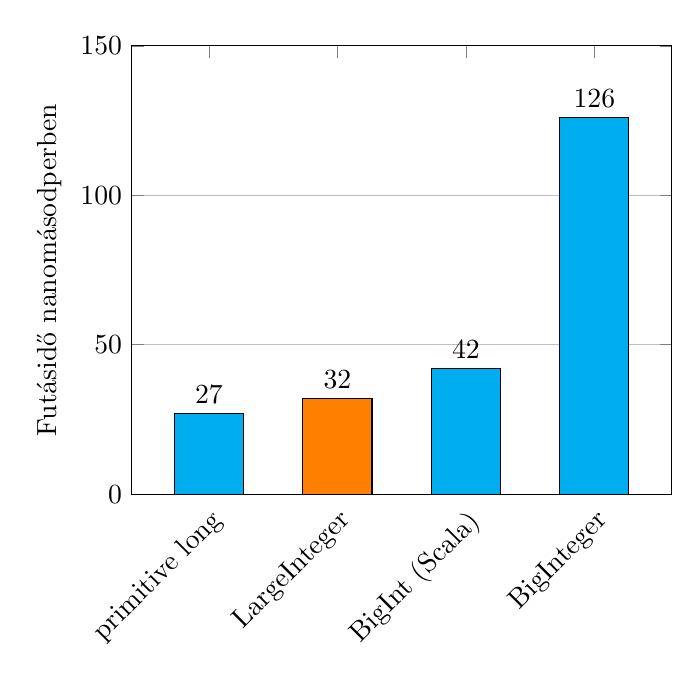
\begin{tikzpicture}
        \begin{axis}[
                symbolic x coords={primitive long,,LargeInteger,,BigInt (Scala),,BigInteger},
                xticklabel style={rotate=45,anchor=north east},
                xtick={primitive long,LargeInteger,BigInt (Scala),BigInteger},
                ylabel=Futásidő nanomásodperben,
                ymajorgrids,
                ymin=0,
                ymax=150,
                bar width=25pt,
                enlarge x limits=0.2,
                nodes near coords,
                nodes near coords align={vertical},
            ]
            \addplot[ybar,fill=cyan] coordinates { (primitive long,27)};
            \addplot[ybar,fill=orange] coordinates { (LargeInteger,32) };
            \addplot[ybar,fill=cyan] coordinates { (BigInt (Scala),42) };
            \addplot[ybar,fill=cyan] coordinates { (BigInteger,126) };
        \end{axis}
    \end{tikzpicture}
    \caption{
        A \texttt{LargeInteger} teljesítményének összehasonlítása
        egy kis számokon végzett összetett számítás átlagos futási ideje alapján
    }
\end{figure}

\subsection{A \texttt{TreeRandom} és implementációi}

Az adatbázist egy hierarchikus képződményként is fölfoghatjuk,
ahol a sémákon belül táblák, azokon belül oszlopok,
azokon belül pedig sorindexekkel megjelölt mezők foglalnak helyet
(vagy egy holisztikus értékkészlet).
Végül a mezők értéke is lehet strukturált adat, melyben a rétegződés folytatódik.
Azt szeretnénk, hogy az értékek bárhol véletlenszerűen álljanak elő,
ugyanakkor determinisztikusan, egy globális kiinduló seed alapján.
Ezért szükségünk van egy olyan véletlengenerátor típusra,
mely teljesíti a következő követelményeket:

\begin{itemize}
    \item tetszőleges számú bitet képes generálni, mindig ugyanazt a (végtelen) bitsorozatot adva vissza
   \item egy kulcs bájtsorozat megadásával visszaad egy alpéldányt (eggyel alacsonyabb szint)
   \item ugyanazzal a kulcs bájtsorozattal egyenlő példányt ad vissza
\end{itemize}

Valamint lehetőleg az alábbi gyenge követelményeket:

\begin{itemize}
   \item véletlenszerű kimenetet ad
   \item eltérő példányoknál jellemzően független, különböző kimenetet ad
\end{itemize}

Az ezeknek való megfelelés a \texttt{TreeRandom} interfészen keresztül történik.

Igen gyakran számokat akarunk előállítani,
ezért kényelmi okokból az interfészhez adtuk a \texttt{getNumber()} default metódust,
mely a paraméterül kapott számnál kisebb nem negatív egészet ad vissza.
Ehhez annyi generált bitet használ,
amennyi a szám elfogulatlan kiválasztásához szükséges (rejection sampling).\footnote{
  Az általános eset miatt valójában egy beépített limittel, melynek elérésekor zérót ad vissza.
  Ha a bitgenerátor-stratégia például csupa 1-est generál
  (ami nem teljesíti ugyan a gyenge követelményeket, de fapados implementációként teljesen valid),
  könnyen végtelen ciklus alakulhatna ki.
}

A fő implementáció hashelésen alapul, és magának a hashelésnek a minőségével skálázható.
Minden ilyen példány belsőleg tartalmaz egy kulcs-bájtsorozatot.
A root példánynál ez a root seed alapján áll elő.
Egy alpéldány előállításakor az eredeti objektum kulcs-bájtsorozatához egy szeparátorbájt,
majd a megadott kulcs alapján előállított bájtsorozat kerül hozzáfűzésre,
így áll elő az alpéldány kulcs-bájtsorozata.

Amikor az adott példányból bitek kerülnek lekérdezésre,
az első néhány bájt a kulcs-bájtsorozat hashelésével áll elő.
A további bitek ennek derivátumai, aminek legegyszerűbb algoritmusa,
ha a hash alapján előállított seeddel inicializált \texttt{Random} példánnyal
rendre visszaadott bájtokat használjuk.

\subsection{A \texttt{Monotonic} és implementációi}

Gyakran egy adott értékkészlet elemeiből akarunk képezni egy $n$ hosszúságú rendezett listát.
Az eloszlás (beleértve, hogy valamely érték egyáltalán előfordul-e)
teljesen implementációfüggő lehet.
Mivel az értékkészlet maga is egy $k$ hosszúsága lista,
a további leképezési kompozíciók szempontjából rugalmasabb,
ha az értékindexeket, azaz a $[0..k)$ egész-intervallum számait tesszūk a listába.

Követelmény, hogy le tudjuk kérdezni az alábbiakat:

\begin{itemize}
    \item egy adott pozícióra mely értékindex került
    \item adott értékindex mely sávba került
\end{itemize}

A rendezettség miatt a második kérdésre mindig egy összefüggő sáv a válasz. Ha az értékindex nem szerepel, akkor ez egy zéróhosszú sáv azon a helyen, ahová a rendezés szerint beszúrható lenne.

Értelemszerűen értéksávokra is tudunk keresni, hiszen az értéksáv szélső értékeinek értékindexeire keresve megkapjuk a képzett sáv széleinek sorindexeit is.

Ezeket az elvárásokat formalizálja a \texttt{Monotonic} interfész.

A legegyszerűbb implementáció a diszkrét lineáris vetítés.
A $k$ hosszúságú értékkészletet ekkor úgy vetítjük az $n$ listahosszra,
hogy az $i$-edik helyre a $\lfloor \frac{k \cdot i}{n} \rfloor$ pozíciójú érték kerül.

A költségesebb, jobb minőségű implementációk pszeudovéletlen mintavételezésen alapulnak.
Ehhez rekurzívan osztjuk föl az értékkészletet, miközben a felosztás fája determinisztikus, mindig ugyanaz.
A fa minden elágazásához tartozik egy mintavételezés, mely eldönti,
hogy az értékkészlet szeletei a céllista mely szeleteire vetüljenek.
A mintavételezéshez jelenleg az Apache Commons Maths könyvtár
\texttt{BinomialDistribution} osztályát használom,
melyet a \texttt{TreeRandom} példányból generált seeddel hívva
determinisztikus eredményt tudok előállítani.

A mintavételezéses eljárás többféleképpen is továbbszofisztikálható.
Egy ilyen lehetőség a szürjektív eredmény biztosítása, amikor szeretnénk, ha minden érték előfordulna
(a zajosan monoton értékkiosztásoknál ennek lesz egy további alkalmazása).
Illetve az is lehetséges, hogy konkrét táblázatunk van,
mely minden értékkészletbeli értékre tartalmazza annak várható előfordulási gyakoriságát.
Ezeket az előre definiált gyakoriságokat használhatjuk a mintavételezésben,
de akár közvetlenül is alkalmazhatjuk egy diszkrét lineáris vetítéssel.

\subsection{A \texttt{Permutation} és implementációi}

Gyorsan számítható invertálható permutációk például modulo szorzásból kiindulva valósíthatók meg.

Költségesebb, de erősen véletlenszerű összevisszaságot biztosító invertálható permutációk
különféle kriptográfiai módszerekkel állíthatók elő.
Többféle algoritmuscsalád kipróbálása után (pl. FPE, azaz Format Preserving Encryption) végül
egy megfelelően kialakított Feistel-hálózat bizonyult a legkezelhetőbbnek.
A Feistel-háló fő skálázási paramétere (akárcsak a hash-alapú \texttt{TreeRandom}-implementációnál)
a hashelő algoritmus minősége,
de a háló mérete illetve a permutáció $n$ hossza is lényeges.

A következő ábrán vizuálisan összehasonlítottam néhány permutáció-típus értékeloszlását
(a közeli értékek színe hasonló; minél összevisszább, annál jobb):

\begin{figure}[H]
  \centering
  \hspace*{\fill}
  \begin{minipage}[b]{0.45\textwidth}
    \centering
    
\includegraphics[width=0.9\textwidth]{image/permutation-fpe1.png}
    \caption{FPE permutáció[hiv!]}
  \end{minipage}
  \hspace*{\fill}
  \begin{minipage}[b]{0.45\textwidth}
    \centering
    
\includegraphics[width=0.9\textwidth]{image/permutation-mp1.png}
    \caption{Modulo permutáció}
  \end{minipage}
  \hspace*{\fill}
  
  \vspace*{0.7cm}
  
  \hspace*{\fill}
  \begin{minipage}[b]{0.45\textwidth}
    \centering
    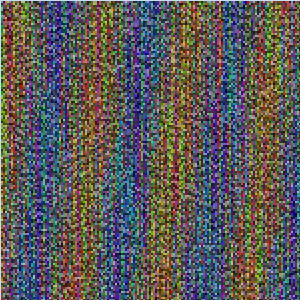
\includegraphics[width=0.9\textwidth]{image/permutation-feif1.png}
    \caption{Feistel-háló (1-round, fast hash)}
  \end{minipage}
  \hspace*{\fill}
  \begin{minipage}[b]{0.45\textwidth}
    \centering
    
\includegraphics[width=0.9\textwidth]{image/permutation-feis2.png}
    \caption{Feistel-háló (2-round, SHA256)}
  \end{minipage}
  \hspace*{\fill}
\end{figure}

A kriptográfiában alkalmazott legtöbb megfordítható permutáció mérete eleve kötött.
A Feistel-háló ebből a szempontból elég rugalmas,
de a permutáció hossza még ekkor is csak 2-hatvány lehet.
A tetszőleges hossz biztosítására átméretező dekorátorok használhatók.
A hosszcsökkentő dekorátor továbbhív a dekorált permutációra,
és ha a kapott érték a célhosszon belül van, akkor visszaadja, ha nem,
akkor a mindenkori értékkel addig hívja újra,
amíg megfelelő értéket nem kap.
A hossznövelő dekorátor ennek felhasználásával implementálható,
de a jelentősége kisebb, jellemzően hosszcsökkentés történik.
Egyes speciális permutációknál az előbbi módszer nagyon sok újrahívással járhat
(például egy olyannál, ahol az értékek eggyel előre tolása történik).
Az átméretező metódus bekerült magába az interfészbe,
hogy az ilyen implementációk maguk kezeljék a helyzetet.
A jó szétszórást biztosító permutációknál valószínűtlen a sok újrahívás.

\subsection{A storage API}

Ha definiáltuk a relációs ontológia fő elemeit,
akkor ezek megfelelő implementációi már megvalósítanak egy relációs adattárat,
mely funkcionálisan megfelel egy tényleges adatbázisnak.
De melyek legyenek ezek az elemek?
A kérdést elsőként a \textit{hozzáférés} szempontjából érdemes megközelíteni.
Az írhatóság problémakörével később foglalkozom.

Nyilvánvalóan gondoskodni kell az alaphierarchiáról,
ezek lesznek a \texttt{Schema}, \texttt{Table} és \texttt{Column} típusok.
Az oszlopok elvont tulajdonságait a \texttt{ColumnDefinition} típus fogja össze.
Bár az egyes mezők értékeit általában oszloporientáltan állítjuk elő,
jellemzően az értéklistákat megadó \texttt{Source} objektumok használatával,
a lekérésnél több szempontból is intuitívabbnak és előnyösebbnek mutatkozik
a rekordorientált megközelítés.
A rekordot a \textt{Row} típus reprezentálja,
ezen keresztül kérhetőek le a konkrét mezőértékek
az oszlopnév vagy oszloppozíció megadásával.

Az adatok hatékony keresését indexek segítik, itt három ilyen indexfajtával fogok foglalkozni,
a normál \texttt{TableIndex}, a \texttt{FulltextIndex} és a \texttt{SpatialIndex} típusokkal.
Ezek keresőmetódusai egy \texttt{TableSelection} példánnyal térnek vissza,
melyen keresztül a találati listához férünk hozzá.

A \texttt{TableIndex} a szokásos rendezett indextípus,
mely egyúttal teljes kontrollal rendelkezik a találati lista rendezése
és a $NULL$ értékek kezelése fölött.
Ha többoszlopos, akkor az oszloplista bármely prefixére is indexként működik (leftmost prefix lookup).

A másik két típus találatainak rendezése definiálatlan.
Egyik sem ad vissza $NULL$ mezőket.

A következő osztálydiagramon a fenti interfészeket foglaltam össze,
a tömörség kedvéért néhol kicsit vázlatosan:

\begin{figure}[H]
\centering
\includegraphics[width=\textwidth]{diagram/storage-api-uml.png}
\caption{A storage API fő interfészei (egy relációs adattár alapontológiája)}
\end{figure}

\section{A csak-olvasható alapréteg}

Bármilyen implementáció legyen is mögötte, a storage API egy relációs adatbázist ír le.
Tehát ahhoz, hogy a virtuális adatok funkcionálisan egy valódi (csak-olvasható) relációs adathalmaz képét adják,
nem kell más, mint hogy megfelelő viselkedéssel elérhetők legyenek a storage API-n keresztül.
A megfelelőség ez esetben két dolgot jelent:

\begin{enumerate}
  \item \textbf{Konzisztencia:}
        felépíthető egy olyan tényleges immutábilis relációs adatbázis ($M$),
        hogy minden lehetséges relációs lekérdezés esetében, amely a közös sémára ($S$) értelmes,
        a virtuális és a tényleges adatbázis esetében visszaadott eredménytábla megegyezik.
  \item \textbf{Megkötések kielégítése:}
        az $S$ séma teljesíti a virtuális adatbázis felhasználói konfigurációját ($C$),
        valamint az $M$-ben szereplő adatok tulajdonságai illeszkednek a $C$-ben leírt megkötésekre.
\end{enumerate}

A virtuális adatokhoz a legalsó szinten a storage API megfelelő hívásaival férünk hozzá.
Ezek a speciális hívások szűk keresztmetszetet képeznek,
hiszen ezek szimulálják például a közvetlen adatelérést is.
Ha ezen hívások performanciája nagyságrendileg (de legalább aszimptotikusan) összemérhető a tényleges adatbázisokéval,
akkor az erre épülő lekérdezésfuttató és egyéb rétegek már
a tényleges adatbázisoknál megszokott módon és nagyságrendi teljesítménnyel tudnak működni.

A lekérdező műveletek esetében két különösen fontos hozzáférési módot kell kiemelni:

\begin{enumerate}
  \item rekordok véletlen elérése (random access)
  \item adott érték előfordulásainak keresése egy oszlopban (reverse index)
\end{enumerate}

Ha e két hozzáférési mód hatékony, akkor már a lekérdezések jelentős részénél
elérhető a tényleges adatbázisokéval összemérhető performancia.

A storage API-ban úgy definiáltuk a \texttt{TableIndex} interfészt,
hogy a keresésen kívül még néhány további funkciót is támogatnia kelljen,
például a rendezést és a $NULL$ értékek kezelését.
Külön kitérek majd az ezzel kapcsolatos problémákra, ahol szükséges.

\subsection{Keretrendszer az értékkiosztásokhoz}

Virtuális adatok alatt elsősorban az egy-egy oszlop alá besorakozó,
közös típussal rendelkező mezőértékeket értem.
Azaz alapesetben, ahogy korábban fogalmaztam, az adatokat oszlop-orientáltan fogjuk előállítani.
Minden oszlophoz tartozik majd egy virtuális adatlista,
melynek hossza egyenlő az adott oszlopot tartalmazó tábla hosszával
(opcionálisan szerepelhetnek benne $NULL$ értékek),
a többi érték típusának pedig kompatibilisnak kell lennie az oszlophoz megadott típussal.

Bár ez a megközelítés oszloponként független adatlistákra van szabva,
valójában más jellegű értékkiosztási módszer is lehet mögötte,
amennyiben az egy-egy oszlophoz tartozó listanézetek biztosítottak.
Majd a több oszlopot érintő megkötések esetében ez lesz a helyzet.
De lássuk először az egyoszlopos értékkiosztások lehetséges módszereit.

\subsection{Indexelt egyoszlopos értékkiosztások}

\subsubsection{Előzetes megfontolások}

Olyan értékkiosztási módszereket veszek most végig,
amelyek lehetőleg biztosítják az alábbiakat:

\begin{enumerate}
  \item hatékony elérés (random access)
  \item pozíciótól függő érték (\texttt{TreeRandom} seed)
  \item hatékony kereshetőség valamilyen formában
  \item hatékony rendezés
  \item konzisztencia
\end{enumerate}

Az egyes esetekben megvizsgálom majd, hogyan teljesíthetők ezek az elvárások.

\subsubsection{$NULL$ értékek kezelése}

Általánosan, bármely értékkiosztási módszerhez könnyen hozzáilleszthető a $NULL$ értékek támogatása.
Mindössze az szükséges, hogy az értékkiosztást a tábla méreténél kisebb intervallumra végezzük,
a maradék helyeket pedig $NULL$-nak tekintjük.
Ezen felül opcionálisan egy permutáció beiktatásával az értékeket elkeverhetjük,
ami által a $NULL$ értékek is szétszórtan szerepelnek majd.

Nem szükséges ez a plusz kompozíció,
ha a fentiek magába az eredeti értékkiosztásba is könnyen beépíthetők.
Például a kétfázisú értékkiosztásokba egyszerűen felvehető a $NULL$ mint érték.

Akár beépítetten, akár plusz kompozícióval van megvalósítva a $NULL$ értékek kezelése,
természetesen figyelni kell a speciális kezelésre a keresés-rendezés során.

A fentiek fényében az egyes értékkiosztások tárgyalásánál a $NULL$ értékek kezelésével nem foglalkozom.

\subsubsection{Egyszerű értékkiosztások}

Tényleges adatbázisokban némely esetben meglehetősen következetes módon
szerepelnek az értékek az oszlop értéklistájában.
Természetesen az ilyen esetek szimulálása a legegyszerűbb.

Triviális eset, ha egy oszlop mezői egy közös konstans értéket tartalmaznak.

Továbbá, ha olyan adathalmazt szimulálunk, melyre megengedhető a feltevés,
hogy nem történt még releváns módosítás
(ami persze az írási réteggel utána korrigálható),
úgy egyes oszlopok szekvenciális alapon generálhatók.
Az ilyen esetekben az $n$-edik érték lekérése
egy egyszerű lineáris függvénnyel számolható.
Az érték keresése hasonló, lényegileg az inverz függvényt kell alkalmazni.

A szekvenciális oszlopoknál az érték megegyezik a rekord 1-től indított sorszámával.

Időbélyegeket is generálhatunk hasonló módon,
amennyiben megengedhető, hogy a szimulált időadatok között egyenletes időközök legyenek.

\subsubsection{Unique értékkiosztás}

Elsődleges vagy más egyedi kulcsok szimulálásakor fontos,
hogy ugyanaz az érték ne forduljon elő kétszer az értéklistában.
Ennek természetesen előfeltétele,
hogy a lehetséges értékkészlet nagyobb legyen, mint az oszlop hossza
($NULL$ értékek nélkül).

Egy egyszerűen megvalósítható módszer,
ha egyszerűen valamilyen \texttt{Permutation} példányt alkalmazunk az értékkészlet fölött,
és a permutált lista oszlophosszúságú prefixét vesszük értéklistaként.
Ekkor a random elérés triviális: csak a permutációt kell visszafejteni.
Az index a rendezett értékkészletre alapozható,
a találatokat a permutációval megforgatva kell listázni,
kihagyva a prefixen kívül eső értékeket.

Ha azonban az értékkészlet mérete lényegesen nagyobb, mint az oszlophossz,
jellemzően nagyon sok értéket kell átugranunk, amely a prefixen kívül esik.
Sokkal hatékonyabb, ha a következő részben leírt általános kétfázisú értékkiosztást használjuk,
ami nem csak unique oszlopokhoz alkalmazható.
A unique oszlop esetén csak annyi a megkötés, hogy a használt \texttt{Monotonic}
a kimenetet szigorúan monoton módon állítsa elő.

\subsubsection{Általános kétfázisú értékkiosztás}

Talán a leggyakoribb eset,
hogy előre ismert véges értékkészlet elemeit szeretnénk viszontlátni az oszlopban,
mégpedig összevissza.

Fentebb már utaltam rá, hogy ez a legtöbb esetben megoldható két független lépéssel.
Először egy \texttt{Monotonic} példány segítségével a kívánt célhosszra
értelmezett függvényt állítunk elő, mely az értékkészlet pozícióira mutat
(ezt a továbbiakban \textit{rányújtás}nak nevezem majd).
Majd az így előállt (esetlegesen $NULL$ értékekkel kiegészített) listát
egy \texttt{Permutation} példány segítségével elkeverjük.

\begin{figure}[H]
\centering
\includesvg[width=0.55\textwidth]{diagram/distribution}
\caption{A kétfázisú értékkiosztás alapelve: egymás után végrehajtott visszafejthető disztribúció és permutáció}
\end{figure}

Láttuk, hogy mindkét függvénytípus interfésze úgy van definiálva, hogy relációként megfordítható.
A \texttt{Monotonic} \texttt{indicesOf()} metódusaival egy értékindexnek illetve -sávnak
a céllistabeli sávjára tudunk rákérdezni.
A \texttt{Permutation} pedig az \textt{indexOf()} metódust biztosítja hasonló célra
(illetve inverze maga is permutáció).
Ezek használatával egy reverse index könnyen implementálható.

A következő két ábra szemlélteti az adatlekérés illetve értékkeresés folyamatát:

\begin{figure}[H]
  \centering
  \hspace*{\fill}
  \begin{minipage}[t]{0.42\textwidth}
    \includesvg[width=\textwidth]{diagram/getvalue}
    \caption{Adatlekérés a kétfázisú értékkiosztásból}
  \end{minipage}
  \hspace*{\fill}
  \begin{minipage}[t]{0.42\textwidth}
    \includesvg[width=\textwidth]{diagram/findvalue}
    \caption{
      Keresés a kétfázisú értékkiosztásban:
      a rendezett értékkészlet és a leképezések megfordíthatósága
      biztosítja a hatékony kereshetőséget a virtuális listában
    }
  \end{minipage}
  \hspace*{\fill}
\end{figure}

\subsubsection{Kétfázisú értékkiosztás gyakoriságtáblázattal}

Egyes esetekben előre ismert az értékek eloszlása,
amit szeretnénk nagyjából vagy pontosan viszontlátni a céloszlopban.
Ekkor egyszerűen a \texttt{Monotonic} fentebb tárgyalt konkrét eloszlásokat használó
implementációnak egyikét kell használnunk.

A felhasználó számára biztosítani kell a gyakoriságok könnyű konfigurálhatóságát.
Ennek legegyszerűbb módja, ha szám-érték párokat kérünk be.
Az értékekhez tartozó számok egymáshoz képesti relatív gyakoriságok.

\subsubsection{Zajosan monoton értékkiosztások}

A rányújtásnak az előzőleg monoton függvény előállításához használt elve
másféle értékkiosztáshoz is felhasználható,
nevezetesen olyan (szigorúan vagy nem szigorúan) monoton adatsor előállításához,
melynek egyes értékei összességében egy adott sűrűség szerint növekednek
(vagy csökkennek; az egyszerűség kedvéért most csak a növekedő esetről lesz szó),
de lokálisan nagy az egyenetlenség.
Ezt is két lépésben fogjuk megvalósítani.\footnote{
  A két lépés általánosítható egy általános sűrűségfüggvény és egy zajfüggvény összegévé,
  ahol a sűrűségfüggvény meredeksége és a zajfüggvény kilengése közötti megfelelő viszonyt kell biztosítani,
  hogy az értékek ne ugorják át egymást.
  Itt most nem foglalkozom ezzel az általánosabb kerettel.
}

Az első lépés alapelve tehát hasonló az előbbi megoldás első fázisához.
Ám itt nem lehetséges értékeket vetítünk ki a tábla hosszára,
hanem a táblahossznyi alaphalmazt vetítjük majd ki egy diszkrét lehetséges értékkészletre.
Minden sorindexhez hozzárendelődik egy (a szigorú monotonitás elvárása esetén nemüres)
dedikált sáv az értékkészletből.

A második lépés választ egy értéket a sávból.
Nem szigorúan monoton értéksor esetén megengedjük az üres sávot is,
és ilyen esetekben mindig a rákövetkező elemet választjuk.\footnote{
  Ebben az esetben explicite ki kell zárni, hogy az utolsó sáv üres legyen.
  Ez legtermészetesebben egy logikai paraméter beiktatásával érhető el,
  amelyet a rekurzió során mindig csak a felsőbb sávra küldünk tovább \texttt{true} értékkel
  (a többire \texttt{false} értékkel),
  alapértelmezett értéke \texttt{true}.
  Ha tehát \texttt{true} értéket kaptunk, biztosítani kell, hogy az aktuális felsőbb sáv ne legyen üres.
}

Az érték elérése ekkor úgy történik, hogy először lekérjük az értéksávot a rányújtó függvénytől,
majd meghívjuk az értékválasztó függvényt,
melynek paraméterei az értéksáv, a sorindex és a \texttt{TreeRandom}-ból vett seed lesznek.
Egy kézenfekvő megvalósítás,
hogy a seed alapján inicializált randomgenerátorral
generáltatunk egy véletlen értéket, ami a sávba esik.

Értéksávra való kereséskor vesszük a minimális és a maximális keresett értéket,
és az inverz rányújtást használva megkeressük a megfelelő sorindexeket, amelyek sávjához az érté tartozik.
Ezen sorindexek feszítik majd ki a találati sorindexsávot.
Hogy az alsó érték beletartozik-e, annak eldöntéséhez le kell generálni
az alső sorindexhez a konkrét értéket, és ellenőrizni, hogy nagyobbegyenlő-e,
mint a keresett alsó érték.
A felső érték esetében hasonlóan kell eljárni.

A rendezés triviális, mivel az értékek eleve rendezettek.

Ezzel az eljárással nem csak zajossá tudtuk tenni az eloszlást,
de a monotonitás garantálása mellett megengedtük,
hogy az értékek esetlegesen csomósodhassanak,
illetve elméletben tetszőlegesen eltávolodhassanak attól a helytől,
amit egy egyszerű, szigorúan egyenletes kiosztás esetén vettek volna föl.

Ez az értékkiosztás különösen alkalmas időbélyegek szimulálására,
amikor az események általános sűrűsége adott,
de véletlenszerű, zajos kimenetet szeretnénk látni.

\subsubsection{Értékkiosztás reguláris kifejezés alapján}

Ha elengedjük a gyors keresés kritériumát,
akkor a reguláris kifejezés alapján történő értékkiosztást nagyon könnyen megvalósíthatjuk
egy véges automatával történő véletlenszerű inverz mintaillesztéssel\footnote{
  A jelenlegi implementáció a \textit{generex} könyvtárat használja erre.
},
a sorindex és a \texttt{TreeRandom}-ból vett seed figyelembevételével.

Ha azonban fenn szeretnénk tartani a gyors keresés lehetőségét,
szükséges lesz, hogy képezni tudjuk az adott reguláris kifejezésre illeszkedő összes string virtuális listáját.
Azaz bármely $n$ sorindexre elő kell tudnunk állítani az $n$-edik illeszkedő stringet
(méghozzá abc-rendben, nem pedig a reguláris kifejezés szerkezete alapján).
És fordítva, tetszőleges stringre meg kell tudni mondani,
hányadik illeszkedő stringgel azonos vagy melyikhez van közel, ha nem illeszkedik.
Ha már van egy ilyen virtuális listánk, azt a kétfázisú értékkiosztással könnyen a kívánt oszloppá alakíthatjuk.

A megoldás a reguláris kifejezések lehetőségeinek csak valamilyen limitált részhalmazát fogja támogatni.
De még így is bőven lefedi az olyan egyszerű eseteket, mint például a telefonszámok, email-címek stb.

Az ilyen típusú szöveggenerálás részletes bemutatása kimutat a jelen dolgozat keretei közül,
így ennek ismertetését itt mellőzöm\footnote{
  Egy egyszerű erre készült prototípus a \texttt{strex} könyvtár.
}.

\subsubsection{Full-text indexelt értékkiosztás}

Ez az értékkiosztási mód folyószövegeket állít elő, melyekhez full-text indexet tesz elérhetővé.
Itt most csak a full-text index legegyszerűbb fajtájával foglalkozunk,
melynek bemenete egy néhány szóból álló halmaz,
eredménye pedig az ezen szavak mindegyikét tartalmazó mezők sorindexeinek halmaza.
Rendezéssel ez esetben nem foglalkozunk, a full-text indexek ezt általában nem is biztosítják.
Látni fogjuk, hogy a bemutatott megoldás könnyen továbbfejleszthető.

Első körben induljunk ki abból, hogy adott egy szólista, a mellékelt $f_i$ előfordulási gyakoriságokkal.
Az $f_i$ előfordulási gyakoriság szimulálható is Zipf törvényére alapozva[hiv!].
A szavakat egyszerűen betűkarakterek sorozataiként fogjuk föl,
előzetesen függetlenítve a központozás, szövegfelépítés problematikájától.

Lesz emellett egy a szövegekre vonatkozó várható szószám is, jelöljük ezt $c$-vel.
A gyakoriság és a hossz együtt meghatározza az adott szó
$p_i$ szereplési valószínűségét valamely szövegben a következő egyszerű képlet szerint:

$$
p_i = 1 - (1 - f_i)^c
$$

Legyen $s$ az egy szövegben várhatóan előforduló szavak halmazának számossága ($s \leq c$).
Az $n$ táblahossz számú mezőre akarjuk képezni a szövegeket,
amit egy $n \times s$ méretű virtuális mátrix segítségével fogunk elvégezni.
A szavakat valamilyen sorrendben véve (a sorrend megválasztásának problémáit most mellőzöm),
az $n s$ hosszú listát feltöltjük úgy, hogy minden szó egy összefüggő sávban szerepel,
a sávok sorrendje az említett szósorrend,
a sávok egymáshoz képesti relatív hossza pedig a $p_i$ szereplési valószínűségen alapul.
Ezt a listát képezzük bele oszlopfolytonosan a mátrixba.

Egy adott sorindexhez tartozó mezőben szereplő szavakat úgy kapjuk,
hogy egyszerűen vesszük a mátrix megfelelő sorát.
Szavakra keresni pedig úgy tudunk, hogy a keresett szavakhoz tartozó
(esetleg oszlopváltással megszakított) sávok metszetsávját vesszük,
ha nincs metszet, nincs találat.
A mátrixsorokat az életszerűség kedvéért érdemes permutálni a fentebb már ismertetett módszerrel.

A mátrixos módszer egyik hátránya,
hogy az egymás mellé került szavak eltartanak egymástól ugyanabban az oszlopban,
így jellemzően nem tudnak majd bekerülni ugyanabba a szövegbe,
illetve általában is viszonylag korlátolt,
hogy melyek a lehetséges konstellációk.
Ez viszonylag jól orvosolható azzal, ha egy-egy szó sávja több független sávba törik szét
(jól ügyelve arra, hogy ezek a részsávok távoli sorokra essenek,
de legalábbis ne legyen metszetük modulo $n$).

Egy másik probléma (hacsaknem épp ez a cél), hogy a szövegek túl uniformak, ugyanannyiféle szóból állnak.
Ezen könnyen segíthetünk, ha a szósávok közé sok apró üres sávot helyezünk el.

A következő ábrák szemléltetik az eddig leírt szóösszeállítási illetve keresési módszert:

\begin{figure}[H]
  \centering
  \hspace*{\fill}
  \begin{minipage}[t]{0.42\textwidth}
    \includesvg[width=\textwidth]{diagram/fulltext-getvalue}
    \caption{Full-text szóösszeállítás}
  \end{minipage}
  \hspace*{\fill}
  \begin{minipage}[t]{0.42\textwidth}
    \includesvg[width=\textwidth]{diagram/fulltext-findvalue}
    \caption{Full-text keresés}
  \end{minipage}
  \hspace*{\fill}
\end{figure}

Egy harmadik egyszerű javítás adódik,
ha előre ismert, mely néhány (ideálisan kb. 6-8) szó lesz gyakran keresve,
ezeket teljesen külön kezelhetjük.
Vesszük az összes lehetséges előfordulási kombinációt azok pontos gyakoriságával,
az így kapott értékkészletet pedig lineárisan rányújtjuk a táblahosszra.
Célszerű ezt a többi szótól teljesen függetlenül permutálni.
Egy mező szóhalmazaként a kétféle kiosztás unióját kell venni,
kereséskor pedig a kettő által adott találatok metszetét.

Megjegyzem, ha vannak kiemelt szavak, akkor a többi szó halmaza részben vagy egészben
akár mesterségesen előállított szavakból is állhat.
Ekkor egy minta alapján generálunk szavakat
(on-the-fly, ld. a reguláris kifejezések kapcsán írottakat),
majd például Zipf törvénye alapján hozzájuk rendeljük a gyakoriságokat.
Ha így járunk el, megspóroljuk a konkrét szavak tárolásának tárhelyigényét.

Egy-egy mezőértékhez még csak a szavak halmazát állítottuk elő.
Amikor lekérjük a mező konkrét értékét, akkor egy tényleges szöveget szeretnénk kapni,
mely pontosan ennek a halmaznak a szavait tartalmazza (sorrendtől és multiplicitástól függetlenül),
és lehetőleg egy viszonylag valóságosnak tűnő szöveg, még ha nem is értelmes.
Vegyük észre, hogy ebben teljes szabadságunk van, hiszen az érték és index konzisztenciája már biztosított.

Az aktuális \texttt{TreeRandom}, a sorindex és a kapott szóhalmaz függvényében
a szöveg generálására tetszőleges módszert használhatunk,
itt tehát egy széles skálázási lehetőség adódik.
A fapados megoldás a halmaz szavainak egyszerű felsorolása szóközzel választva
(abban a sorrendben, ahogy a kiemelt szavak fel voltak sorolva, illetve ahogyan a mátrixból nyertük őket).
Egy nagyon szofisztikált módszer lehet, ha nyelvi modellt használunk a szöveg generálására.

Egy olcsó, ugyanakkor viszonylag jó eredményt adó módszer a következő:

\begin{enumerate}
    \item Határozzuk meg a $c_i$ konkrét szószámot.
    \item Vegyük a szóhalmazt valamilyen konkrét sorrendben.
    \item Helyezzünk ezek közé további szavakat, míg a $c_i$ szószámot el nem érjük.
    \item Határozzuk meg a mondat- illetve részmondathatárok pozícióit.
    \item Fűzzük össze a szöveget szóközökkel, adjuk hozzá a központozást.
\end{enumerate}

Mindegyik lépés finomítható különféle heurisztikákkal,
ezekkel most nem foglalkozom.

A fent tárgyalt full-text index természetes módon bővíthető.
Könnyen integrálható például a kizárandó szavak kezelése.
A szóhalmaz kiválasztásának és a szöveg generálásának összehangolásával
a kifejezésekre való keresés bizonyos formái is megvalósíthatóvá válnak.
Ezekre a bővítési lehetőségekre ezen keretek között szintén nem tudunk részletesen kitérni.

\subsection{Földrajzi koordináták értékkiosztása}

A legegyszerűbben közelítjük meg a problémát,
ami nagyobb dimenziószámra és lényegileg tetszőleges geometriára is átvihető.
Csak a megoldás vázát ismertetem.

Az értékek sűrűségének, elhelyezkedésének valamint opcionálisan a várható lekérdezések
figyelembevételével a felületet térszeletekre osztjuk.
Ennek a felosztásnak nem feltétlenül kell egyenletesnek vagy egyáltalán szabályosnak lennie,
de az egyszerűség kedvéért most maradjunk a szokványos hálónál:
adott $w$ földrajzi hosszúságonként illetve adott $h$ földrajzi szélességenként vágjuk föl a gömbfelszínt.
A kapott háló (a sarkoknál háromszöggé fajuló) kis kvázi-négyszögeket határoz meg.
Ezeket soronként véve egy lineáris sorrendezést kapunk.

A szélesség-hosszúság párokat egy $2d$ bites ábrázolással kódoljuk.
Ennek lehetséges értékkészletére nyújtjuk rá a sorindexeket
a zajosan monoton értékkiosztásoknál ismertetett módszer valamely variánsával,
de itt a nagyléptékű egyenletességet más szempontokra cserélhetjük.
Az értékkészlet összefüggő sávjai a kvázi-négyszögeknek feleltethetők meg,
tehát a kvázi-négyszögekbe tartozó értékekre ugyanúgy tudunk keresni,
mint fentebb az időbélyegekre.

Kereséskor a kvázi-négyszögek két halmazát kell elkülöníteni:
amelyek teljesen az alakzaton belülre esnek,
illetve amelyeket az alakzat határvonala átmetsz.
Az előbbiek értékei feltétel nélkül találatok lesznek.
Utóbbiaknál a kvázi-négyszögön belülre kell hatolnunk,
esetleg egyesével kell ellenőriznünk az értékek alakzaton belüliségét.
Mivel ezek a határvonalhoz köthetők,
számuk egyszerű alakzatok esetén a kerülettel egyenesen arányos,
nem kell tehát területarányos mennyiségű kvázi-négyszöget megbontani,
sőt, az egy sorban egymás után lévők összevontan is kezelhetők.

\begin{figure}[H]
\centering
\includesvg[width=0.7\textwidth]{diagram/geospatial-search}
\caption{
  Geolokációk keresése alakzat alapján, rácsozott gömbfelületen. \\
  Csak a határvonal által metszett mezőkbe eső pontokkal kell részletesebben foglalkozni.
}
\end{figure}

\subsection{Nem-indexelt egyoszlopos értékkiosztások}

A nem-indexelt oszlopok szimulálásakor a keresési-rendezési szempontokat egyáltalán nem kell figyelembe venni.
Az indexelt oszlopokra vonatkozó elvárások közül így csak az első kettő releváns:

\begin{enumerate}
  \item hatékony elérés (random access)
  \item pozíciótól függő érték (\texttt{TreeRandom} seed)
\end{enumerate}

Vagyis elég, ha a \texttt{TreeRandom} által a sorindexhez generált seed alapján
előállítunk egy normál \texttt{Random} példányt,
és ennek felhasználásával a tartalmat tetszőleges determinisztikus módszerrel állíthatjuk elő.
Erre az előállításra kizárólag a konfigurációban megadott beállítások jelentenek megszorítást.

A következő listában csak fölvillantanám az ilyen adattartalmak néhány jellegzetes,
egyúttal könnyen szimulálható típusát:

\begin{itemize}
  \item \textbf{Egyszerű szöveg:}
    a legegyszerűbb megoldásban egy szótár szavait véletlenszerűen helyezzük egymás után,
    közben feljavítva a szövegképet nagybetűs szavakkal és központozással
    (az eredmény tovább javítható kifejezésminták használatával,
    amikor időnként egy többszavas részletre előre adott sablont használunk;
    de ha a minőség az elsődleges, bevethetünk Markov-láncokat[hiv!] vagy különféle nyelvi modelleket)
  \item \textbf{Strukturált szöveg:}
    először előállítunk egy általános struktúrát (címek, bekezdések stb.),
    majd ennek elemeit feltöltjük szöveggel (lásd az előző pontot),
    végül a struktúrát a kívánt jelölőnyelven szolgáltatjuk (HTML, MarkDown, plain text stb.)
  \item \textbf{Strukturált adat:}
    generált vagy konfigurációban megadott adatséma alapján rekurzívan generáljuk le az adatstruktúrát,
    ekkor a sémanyelv (pl. JSON Schema) és a kimenet formátuma (JSON, YAML, TOML stb.)
    függetlenül konfigurálható
  \item \textbf{Egyszerűbb képek:}
    véletlen színű háttérre véletlen paraméterekkel
    rárajzolunk néhány egyszerű alakzatot,
    majd a kívánt vektoros vagy raszteres formátumban szolgáltatjuk
  \item \textbf{Jelszó-hash:}
    a tényleges a hash-algoritmust hívjuk meg valamely rendelkezésre álló adatra,
    pusztán formai elvárás esetén akár magára a \texttt{TreeRandom} seedre,
    demózáshoz pedig hasznos lehet a felhasználóvet használni jelszóként
  \item \textbf{Általános BLOB/CLOB:}
    lekéréskor a konfigurációban megadott mérethatárok közötti bájtsort/karaktersort kell visszaadni,
    ami könnyen ellátható random bájtok/karakterek generálásával
    (legegyszerűbb közvetlenül a \texttt{TreeRandom} által szolgáltatott biteket használni)
\end{itemize}

További indexeletlen eset, amikor az oszlop teljes tartalma explicite felsorolva van megadva,
például egy listafájlból.
Nagy táblahossznál érdemes lehet ezt indexeltté tenni egy tényleges adatstruktúrával (például B-Tree),
mivel ilyenkor valószínűleg úgysem a memóriahasználat minimalizálása a cél.

\subsection{Értékkiosztás oszlopok közötti összefüggéssel}

Az oszlopok közötti összefüggésnek számtalan módja lehetséges.
A legáltalánosabb eset képletszerű összefüggések felsorolása lenne,
ami indexeletlen esetben meg is megvalósítható:
a \texttt{TreeRandom}-ból nyert seeddel véletlenszerűsítve futtathatunk valamilyen constraint solvert,
mely a követelményeket teljesítő értékeket determinisztikusan előállítja.
Ha lehetséges, hogy egyes seed értékek mellett a követelményrendszer nem kielégíthető,
akkor meg kell engednünk a $NULL$ értékeket az érintett oszlopokban,
és a kielégíthetetlen esetekben mindegyikre $NULL$-t kell visszaadni
(esetleg valamilyen egyéb alapértelmezett értéket).

Szintén elég általános eset, amikor mesteroszlopok
alapján akarunk indexeletlen oszlopokat egymástól függetlenül legenerálni.
Ekkor teljes szabadságunk van,
értelemszerűen a mesteroszlopok értékei és a \texttt{TreeRandom}-ból nyert seed lesz a bemenet.

Életszerű azonban, hogy indexelt mesteroszlopokon túl
a függő oszlopokra is szeretnénk indexelést.
Ha egy nagy közös index elég,
akkor elégséges a függő értékeket becsoportosítani a mesterértékek alá.

Bonyolult, de még mindig teljesen életszerű eset,
amikor a függő értékek külön önálló indexeket is kapnak
(ilyen eset például, ha az életkor adatot a végzettséghez igazítva generáljuk).
Ha a mesteroszlop(ok) értékkészlete kicsi,
akkor minden ilyen értéken belül elvégezhetjük a keresést illetve rendezést a függő értékekre,
és ezek összefésült eredményét adjuk vissza.

\subsection{Táblák közötti kapcsolatok}

Amíg megmaradunk a read-only szempontoknál,
a táblák közötti idegenkulcs jellegű kapcsolatokra vonatkozó egyetlen kemény követelmény,
hogy a hivatkozó tábla érintett oszlopa (vagy oszlop-$n$-ese)
csak a hivatkozott tábla érintett oszlopának (vagy oszlop-$n$-esének) 
értékkészletének elemeit vehesse föl.
Vagyis ($NULL$ értékektől eltekintve),
a hivatkozó oszlop értékkiosztásakor az alaplista a hivatkozott oszlop tartalma lesz.
Másként fogalmazva, az értéklistát indextartó módon kell átképezni a másik táblára.
Ez a fentiek tükrében már egyszerűen biztosítható.

Egyes esetekben (bizonyos típusú 1:1 kapcsolatok) valójában egy tábla kerül szétbontásra több táblára.
Ekkor a több táblára bontottság csak külsődleges,
és az előző részben oszlopok közötti összefüggésekről írottak alkalmazhatók,
még akkor is, ha a két tábla számossága nem egyezik teljesen
(a hiányzó sorok a $NULL$ értékek kezelésének fentebb ismertetett
általános módszerével kerülhetnek kiválasztásra).

A legbonyolultabb esetben 1:n kapcsolat mellett különféle statisztikai
vagy egyéb követelményeket biztosító indexelt oszlopokat szeretnénk előállítani.
Ennek tárgyalása messzire vezet,
de egy rövid megjegyzéssel érzékeltetném, hogy a dolog nem lehetetlen:
egy lehetséges kiinduló megközelítés, hogy a két táblát egyként kezeljük,
az egyesített táblában a kisebb tábla adatait pedig redundánsan szerepeltetjük
(ez egy oszlopközi összefüggés a fenti értelemben);
így az összefüggéseket már táblán belül tudjuk értelmezni.

\section{Az írhatósági réteg}

\subsection{A \texttt{DiffTable} dekorátor}

A virtuális adattár egy-egy példánya várhatóan viszonylag rövid élettartamú lesz.
Feltehetjük, hogy az írási műveletek összességében kevés módosítást eredményeznek.
A tipikus szcenáriókban főként egyes konkrét rekordok lesznek módosítva, hozzáadva, törölve.
A tömeges módosítások kérdésével itt nem foglalkozom,
de nem látszik akadálya az ezek optimalizálását célzó továbbfejlesztésnek.

Az írhatósági réteget arra is használhatjuk,
hogy egy-egy tesztesethez egyéni rekordokat adjunk hozzá,
ami megkötéseken keresztül nehézkesebb lenne.

A módosítások támogatásához előszöris a \texttt{Table} interfészt magát
ki kell egészíteni a megfelelő műveletekkel
(pl. \texttt{isWritable()}, \texttt{applyPatch(TablePatch)}, \texttt{sequence()}).
A csak-írható implementáció persze az írási műveleteket nem fogja támogatni.

A \texttt{DiffTable} egy tetszőleges \texttt{Table} implementáció fölé elhelyezhető dekorátor.
Teljesen áttetszően működik: amíg nincsenek módosítások,
minden műveletet egyszerűen továbbít a dekorált tábla felé.
Módosítás esetén a különbségeket (módosított értékek, beszúrt és törölt sorok) a memóriában tárolja.
A további lekérdezésekkor figyelembe veszi a különbségréteget a továbbhíváskor,
illetve a szükséges mértékben összefésüli az eredményt a különbségekkel.

Olyan táblák is dekorálhatók így, amelyek valós adatbázistáblákat használnak backendként.
Ezzel a módszerrel írhatóan használhatunk egy létező adatbázist,
az eredeti adatok módosítása nélkül.

\subsection{Generikus tranzakciókezelés}

A fő elv, amit a tranzakciókkal kapcsolatban követni fogunk,
hogy megmaradjunk a réteges felépítésnél,
és semmiképp ne a táblákra terheljük a tranzakciókezelés terhét
(mint számos adatbáziskezelő architektúrájában láthatjuk[hiv!]).

Egy teljesen általános tranzakciókezelési módszer,
amikor a szerver két állapotát különböztetjük meg,
a \texttt{READ} és a \texttt{WRITE} státuszokat.
Feltételezzük, hogy jóval több olvasási kérés érkezik be, mint írási.

Az alapértelmezett \texttt{READ} státuszban feltétel nélkül, konkurrensen
szolgáljuk ki a beérkező olvasási lekérdezéseket.
Ha azonban egy módosító lekérdezés illetve tranzakció érkezik,
elhelyezzük a módosító műveleteknek fenntartott queue-ba,
és átváltunk \texttt{WRITE} módba.

\texttt{WRITE} módban a beérkező olvasási illetve írási műveletek
a számukra fenntartott két dedikált queue-ba kerülnek.
Először kiszolgáljuk a még folyamatban lévő olvasási műveleteket,
ezután sorra szekvenciálisan kivesszük és végrehajtjuk a módosítási queue elemeit, amíg van ilyen.
Ha már nincs elem a módosítási queue-ban,
akkor az olvasási queue összes elemét felszabadítjuk, és továbbítjuk párhuzamos végrehajtásra,
miközben visszaállítjuk a \texttt{READ} státuszt.

Új módosító művelet érkezésekor a ciklus újrakezdődik.

\subsection{Snapshot-alapú tranzakciókezelés}

A \texttt{DiffTable} dekorátor minden további nélkül elhelyezhető
más \texttt{DiffTable} objektumok fölé is, ami lehetővé teszi, hogy egymásra épülő snapshotokat tároljunk.

Így könnyen megvalósítható a \textit{multiversion concurrency control} (MVCC),
amikor a kiinduló állapot snapshotja a módosító műveletek közben is rendelkezésre áll,
azaz az olvasási műveletek ekkor is zavartalanul futtathatók.
Az írási tranzakció végeztével az érintett \texttt{DiffTable} példányok
beküldik a saját módosítási rétegüket a dekorált táblába,
így az belefésülésre kerül a megosztott adattérbe.

A snapshotok alkalmazásából a tranzakciós savepointok támogatása is természetesen következik.
Egy savepointra való visszaugrás egyszerűen a megfelelő szintre való visszatérést jelenti
a \texttt{DiffTable} dekorátorok egymásra épülő hierarchiájában.

Mivel a snapshotkezelés táblánként függetlenül működtethető,
párhuzamosan is futtathatunk írási tranzakciókat,
amíg azok különböző táblákon futnak.


\chapter{Gyakorlati eredmények}

\section{A prototípus}

\begin{figure}[H]
\centering
\includesvg{diagram/simplearch}
\caption{A virtuális adatbázis vázlatos architektúrája}
\end{figure}

A virtuális adatbázist megvalósító szoftvert HoloDB néven tettem elérhetővé.
Az elnevezés a hologramokra utal:
a konfigurációból leképzett, ``kivetített'' virtuális adatbázis hasonlóan illuzórikus,
mint a hologramból előhívott térbeli látvány.

A HoloDB sok tekintetben már kinőtte a prototípus státuszt,
hiszen egy nagyívű rétegelt architektúráról van szó,
mely kellően megszilárdult alapvonalakkal rendelkezik a hosszútávú fejlesztéshez.
Ugyanakkor stabil verzióról még nem beszélhetünk;
az implementációs részleteket, valós használati eseteket,
más eszközökkel való integrációt illetően még számos felmérendő, kikísérletezendő dolog adódik.

A szerver docker konténerként is futtatható, amihez a Docker Hubon biztosítok egy testreszabott képet.
A felhasználói Dockerfile mellé csak a konfigurációs fájlt kell elhelyezni az indításhoz.
A testreszabott kép a kis erőforrásigény miatt serverless végpontként is jól használható.\footnote{
    Későbbi terv egy erősen optimalizált, GraalVM-re épülő képváltozat fejlesztése.
}

A HoloDB a MiniBase projektre épül.
Utóbbi egy relációsadatbázis-keretrendszer, mely definiálja a storage API-t,
és annak konkrét implentációjához agnosztikusan viszonyulva
egy komplett adatbázisszervert épít fölé;
beleértve a lekérdezések fordítását és futtatását,
a felhasználói munkamenetek, tranzakciók és változók kezelését,
a runtime sémamódosításokat illetve új táblákat és más felelősségi köröket.
A HoloDB ehhez a storage API virtuális implementációját,
a konfiguráció kezelését
és a megfelelő futtatási környezetet adja hozzá.

A MiniBase közvetlenül biztosít egy SQL-futtató felületet, a MiniConnect API megvalósításával.
A MiniConnect testvérprojekt célja egy egyszerű és egyértelmű adatbázis-elérési API definiálása,
melyet a JDBC nehézkessége inspirált.\footnote{
    Nem áll módomban ehelyt a JDBC részletes kritikájába bocsátkozni.
    De milyen problémát is old meg a \texttt{nativeSQL()} metódus?
    Egyáltalán miként egyszerűsítené a helyzetet ez a kellemetlenül rengeteg függvény?
    Miért származik a \texttt{PreparedStatement} a \texttt{Statement} típusból?
    Hosszan folytathatjuk a sort.
}
A MiniConnecthez különféle middleware változatok is elérhetők, például hálózaton keresztül is használható,
illetve letisztultsága miatt könnyen írhatók hozzá dekorátorok, proxyk.
Egy (deb csomagként is elérhető) REPL is tartozik hozzá,
mellyel parancssorból tudunk hálózaton keresztül csatlakozni a MiniConnectet támogató tetszőleges adatbázishoz.
Ez egyúttal a HoloDB kipróbálásának legkényelmesebb módja,
számos kényelmi funkciót támogat (szép kimenet, syntax highlight, parancstörténet stb.).

Az architektúra köré sokféle további eszközt fejlesztettem,
melyek a robusztusság eltérő fokain állnak.
Ilyenek például: automatikus REST API, GraphQL adapter, authentikációs proxy, Apache Calcite SQL driver stb.

\section{Konfiguráció}

A HoloDB egy YAML formátumú konfigurációs fájl segítségével paraméterezhető fel,
melyben az adatbázis minden lényeges eleme beállítható.
A konfigurációhoz formális specifikáció is tartozik,
így a fájl strukturális és szemantikai helyessége statikusan ellenőrizhező.
A konfigurációt hordozó Java-osztályok egy programkódban is használhatók,
ez csak egy dedikált, minimalisztikus csomag függőségként való beemelését igényli.

\begin{figure}[H]
  \centering
  \begin{minipage}[t]{0.45\textwidth}
    \begin{Verbatim}[frame=single,fontsize=\small]
seed: 425364
schemas:
  - name: shop
    tables:
      - name: customers
        size: 5
        columns:
          - name: id
            mode: COUNTER
          - name: firstname
            valuesBundle: forenames
          - name: lastname
            valuesBundle: surnames
          - name: birth
            valuesRange: [1950, 2000]
      - name: orders
        size: 12
        columns:
          - name: id
            mode: COUNTER
          - name: cid
            valuesForeignColumn: [
              customers, id]
          - name: product
            valuesBundle: fruits
          - name: quantity
            valuesRange: [1, 10]
    \end{Verbatim}
  \end{minipage}
  \hspace*{\fill}
  \begin{minipage}[t]{0.4cm}
    \vspace{6cm}
    {\Large $\Rightarrow$}
  \end{minipage}
  \hspace*{\fill}
  \begin{minipage}[t]{0.45\textwidth}\begin{center}
  
    \vspace{0.8cm}
    
    \texttt{customers}
    \vspace{0.1cm}
  
    \begin{tabular}{ |r|l|l|r| }
      \hline
        \multicolumn{1}{|>{\centering\arraybackslash}m{6mm}|}{\textbf{\texttt{id}}} &
        \multicolumn{1}{>{\centering\arraybackslash}m{18mm}|}{\textbf{\texttt{firstname}}} &
        \multicolumn{1}{>{\centering\arraybackslash}m{18mm}|}{\textbf{\texttt{lastname}}} &
        \multicolumn{1}{>{\centering\arraybackslash}m{12mm}|}{\textbf{\texttt{birth}}} \\
      \hline
        1 & Howard & Anderson & 1968 \\
        2 & Rebecca & Ferguson & 1959 \\
        3 & Jeremy & Moore & 2000 \\
        4 & Julie & Ellis & 1951 \\
        5 & Kathleen & Cook & 1971 \\
      \hline
    \end{tabular}
    
    \vspace{1cm}
    
    \texttt{orders}
    \vspace{0.1cm}
    
    \begin{tabular}{ |r|r|l|r| }
      \hline
        \multicolumn{1}{|>{\centering\arraybackslash}m{6mm}|}{\textbf{\texttt{id}}} &
        \multicolumn{1}{>{\centering\arraybackslash}m{9mm}|}{\textbf{\texttt{cid}}} &
        \multicolumn{1}{>{\centering\arraybackslash}m{18mm}|}{\textbf{\texttt{product}}} &
        \multicolumn{1}{>{\centering\arraybackslash}m{16mm}|}{\textbf{\texttt{quantity}}} \\
      \hline
        1 & 5 & date & 10 \\
        2 & 2 & orange & 1 \\
        3 & 2 & sloe & 2 \\
        4 & 3 & melon & 7 \\
        5 & 5 & guava & 9 \\
        6 & 3 & orange & 6 \\
        7 & 2 & plantain & 3 \\
        8 & 4 & pear & 7 \\
        9 & 4 & papaya & 9 \\
        10 & 5 & line & 9 \\
        11 & 3 & sloe & 4 \\
        12 & 1 & strawberry & 1 \\
      \hline
    \end{tabular}
    
  \end{center}\end{minipage}
  \par
  \caption{Egy minimalisztikus konfiguráció és eredménye}
\end{figure}

A konfiguráció ezen kívül JPA-entitásokra helyezett annotációkkal is beállítható,
így külső eszközök nélkül is futtathatunk teszteket beágyazott adatbázissal.

Az egyéni működéssel való kiegészítés több szinten támogatott.
A beépített értékkiosztási módok esetén is lehetőség van egyéni adatfájl betöltésére,
a permutációk és rányújtások egyéni implementációjának betöltésére.
De az oszlop értékkiosztásához teljesen egyedi implementáció is használható,
ehhez meg kell adnunk egy olyan osztály nevét, mely implementálja a \texttt{SourceFactory} interfészt
(illetve biztosítani kell, hogy az egyedi osztályok láthatóak legyenek a classpath alatt).

A YAML formátum a humán kezelhetőségen kívül azzal az előnnyel is jár, hogy könnyen előfeldolgozható.
Például egy megfelelő sablonkezelő használatával ugyanazt a vázat használva
különféle tesztesetekhez finomhangolhatjuk az adatbázist.\footnote{
    Ilyen megközelítést használ például a \textit{helm} nevű deployment eszköz.
}

A konfiguráció gépileg is generálható.
A prototípus tartalmaz néhány ilyen segédeszközt,
ezek közül a legfontosabb a konfigurációt a meglévő adatbázis letapogatásával,
különféle heurisztikák bevetésével legeneráló, Python nyelven írt szkriptfájl.
Az eredmény (és persze maga a szkriptfájl is) könnyen testreszabható.

Ahogy már említettem, a konfiguráció szofisztikáltabb generálásának egy lehetséges módja,
ha a konfigurációt optimalizáló mesterséges intelligenciára épülő módszert vetünk be.
Ennek kutatása egy izgalmas jövőbeli projektnek ígérkezik.
Érdekes probléma például, hogyan érdemes számítani a bemeneti adatbázis
és az előállított konfiguráció közötti megfelelőségi mutatót.

A konfigurációs fájl az adatbázis nagyjábóli definíciójának is felfogható.
Egy másik ígéretesnek tűnő továbbfejlesztési lehetőség,
hogy kiegészítsük a struktúrát olyan további opcionális elemekkel,
melyek egyrészt teljesen leírják az éles adatbázis szerkezetét,
másrészt pedig lehetővé teszik az adatmigrációknak
kizárólag a konfigurációs fájlok különbségén alapuló automatizálását.
Természetesen ez egyáltalán nem triviális,
hiszen néha a meglévő adatok átstruktúrálására van szükség,
illetve lehetnek a két konfigurációs állapot közötti történetben elbújó lényeges módosítások.
Úgy vélem, mindkét probléma kezelhető,
közeljövőbeli tervem egy ilyen migrációs keretrendszer kialakítása.

\section{Néhány bővítési példaszcenárió}

Eddig általános igényekkel foglalkoztunk,
melyeket a megoldásnak out-of-the-box kell támogatnia.
Alább bemutatok három speciálisabb szcenáriót,
demonstrálva az architektúra bővíthetőségét és rugalmasságát.

\subsection{Valós címadatok használata}

Előfordulhat, hogy bizonyos adatok óriás értékkészletét külső adattárakból szeretnénk betölteni,
amivel ugyan elvesztjük a teljes virtualitás kis memóriaigényét és további kedvező jellemzőit,
de még mindig igényt támaszthatunk az egyéb előnyökre.
Most egy ilyen szcenáriót vizsgálok meg:
valamely tábla rekordjaiban olyan magyarországi közigazgatási címeket szeretnénk viszontlátni,
melyek valósak.
Amennyire lehetséges, indexeket is szeretnénk biztosítani.

A cím elemei különálló mezőkre bonthatók.
Első körben kiválasztjuk azokat, melyek egy egyértelmű hierarchiát definiálnak:

\begin{center}
    településnév ~ $\rightarrow$ ~
    kerület ~ $\rightarrow$ ~
    közterület neve ~ $\rightarrow$ ~
    közterület jellege ~ $\rightarrow$ ~
    házszám ~ $\rightarrow$ ~
    egyéb
\end{center}

Az ``egyéb'' részt nem szofisztikáljuk tovább, egy szabad szöveges mezőnek tekintjük.

Néhány további mező nem tartozik a fő hierarchiába:

\begin{center}
    település típusa ~ $\bullet$ ~
    vármegye ~ $\bullet$ ~
    irányítószám
\end{center}

Utóbbi mezőkre külön-külön indexeket fogunk biztosítani.
A fő hierarchiára pedig egy közös többoszlopos (leftmost prefix) indexet,
pontosabban kettőt:
lesz egy rövidített változat vidéki címekhez, melyben a kerületet nem kell megadni,
és implicite üres értékkel töltődik, amikor továbbhív a másik indexre.

A címadatbázist egy nagy fastruktúrába rendezzük,
minden szintnek a fenti hierarchia egy-egy eleme felel meg.
Az alsóbb szinteken spórolhatunk a tárolással,
például egymásutáni megbontatlan házszámok tartományként tárolhatók.
Egy prefix indexhívásnál a megfelelő szintig megyünk le a keresésben,
a találatok pedig az az alatti levelek lesznek.
A tényleges rekordokra való leképezést
a kétfázisú értékkiosztásnál megismerthez hasonló módszerrel végezzük el.

A fő hierarchián kívüli mezők értékei és a fa közötti indexelést külön adatstruktúrába generáljuk.
Változó lehet, hogy a tábla mely szintjén történik meg az irányítószámra való leképezés,
a legtöbb helyen egy egész várost tudunk hozzárendelni.

\subsection{Valószerű geográfiai értékek előállítása}

A probléma: földrajzi koordinátákhoz akarunk valamilyen számszerű adatot kapcsolni úgy,
hogy mindkettőhöz külön index tartozik,
és a koordinátával ellátott adatok valamilyen szempontból valószerű elrendeződést mutatnak.
Olyan megoldást kell találni, ahol tetszőleges számú ilyen kapcsolt adat akár függetlenül generálható
(különben elég lenne a szélesség-hosszúság-adat háromdimenziós terében megfelelően alkalmazni
a földrajzi koordináták fentebb ismertetett értékkiosztását).

Az alapötlet rendkívül egyszerű, és kellően rugalmas.
Szükségünk lesz egy $F$ függvényre, mely minden földrajzi koordinátához rendel egy kapcsolt értéket.
A kapcsolt adat értékkészletét kis sávokra bontjuk föl (nevezzük ezeket kontextussávoknak),
és minden sávhoz le kell tudnunk kérni azon alakzatok (véges) listáját,
melyekben az $F$ függvény értéke a sávba esik.
Bármilyen függvény megfelel, ha ezeket tudjuk biztosítani hozzá.
Használhatunk például teljesen virtuális háromszögelt felületet,
ahol egy-egy háromszög mindig egy konkrét értéksávba esik, nem nyúlik át.
Vagy akár betölthetünk tényleges domborzati adatokat.

Ha ezt sikerült megoldani, az értékkiosztás működése már triviális.
Adott rekordhoz a földrajzi koordinátát a korábban ismertett módszerrel generáljuk,
a kapcsolt adatot ez alapján számítjuk az $F$ függvény szerint.
A kapcsolt adat valamely egyéni értéksávjára való kereséskor
lekérjük a sávon teljesen belülre eső illetve a kilógó kontextussávokat,
lekérjük az ezekhez tartozó alakzatokat,
és ezen alakzatokra keressük a földrajzi koordinátákat.
A keresett sávon teljesen belülre eső kontextussávokhoz tartozó találatok feltétel nélkül megtarthatók.
A kilógó kontextussávokban le kell kérni a konkrét kapcsolt értéket,
és eldobni a találatot, ha az mégsem esik a keresett sávba.

\subsection{On-demand schema}

Egyes használati esetek megengedik,
hogy további drasztikus lépésként teljesen nyitottá és automatikussá tegyük a virtuális adatbázis felépítését.
Ebben az esetben konfigurációs fájl létrehozására sincsen szükség,
mindent a beérkező kérések alapján fogunk generálni.
Itt feltételezem, hogy csak olvasási műveletek érkeznek,
de az elv, komoly komplikációk vállalásával, írható műveletekre is kiterjeszthető.

Néhány alapbeállítást (pl. \texttt{seed}) beégethetünk, vagy az első lekérés függvényévé tehetünk.

A táblás lekérések implicite megadnak valamilyen szerkezetet,
mivel konkrét sémákon és táblákon belüli konkrét oszlopokat próbálnak elérni.
Ezeket on-demand kell létrehozni, és a továbbiakban megtartani.
A táblák hosszának beállításakor esetleg figyelembe vehetjük az első lekérés limit értékeit, ha van.
Az oszlop paramétereit a lekérésben az adott oszlopra vonatkozó
implicit információk alapján kell meghatároznunk.
Az oszlopnév, az érték használati módja, a keresési feltételek stb.
mind hasznosak lehetnek.
Ha nem tudtuk eléggé leszűkíteni az oszlop típusát,
valamilyen kellően generikus alapértelmezett beállítást kell használnunk,
ekkor is vállalva persze, hogy egy jövőbeli lekérdezés ezzel inkompatibilis lesz.

A wildcardos lekérdezéseknél többféle stratégiát követhetünk,
legegyszerűbb, ha egyszerűen az addigi oszlopokat adjuk vissza
(új tábla esetén egy alapértelmezett oszlopot adhatunk hozzá).

A szisztéma megvalósításához mindössze egy proxy réteg szükséges,
mely minden beérkező kérés továbbítása előtt megfelelően kiegészíti a konfigurációt,
és újratölti a virtuális adatbázist.

\section{Empirikus eredmények}

A három jól elkülöníthető adatbázis-szolgáltatási móddal
(adatgenerálás, anonimizálás, virtuális adatbázis)
megvalósítottam ugyanannak a demó alkalmazásnak a tesztkörnyezetét,
és ezen integrált tesztek egy gyűjteményét futtattam le,
mérve többek között a preparálási, indítási, runtime, és összesített performanciát,
illetve a memóriahasználatot.
A tesztben csak a beépített alaképességeket vettem igénybe,
melyek idiomatikusnak tekinthetők a HoloDB szempontjából,
ugyanakkor egy valószerű szituációt igyekeztem modellezni.

\begin{center}
  \setlength{\unitlength}{1cm}
  \begin{picture}(12,9)(0,0)
    \setlength\fboxsep{0pt}
    \colorbox{gray!20}{\framebox(12,9){[TODO] Ábra: Teljesítményteszt eredménye három megközelítéssel}}
  \end{picture}
\end{center}

Látható, hogy összesített performanciában és memóriahasználatban a HoloDB
nagyságrendekkel jobban teljesít, épp ahogyan azt vártuk.
A vizsgált valószerű szituációban a runtime performancia is
alig marad el a tényleges adatbázisok mögött.

\section{Konklúzió}

A dolgozatban az adatbázismockolás egy újszerű megközelítését mutattam be.
Láthattuk, hogy néhány alapvetően egyszerű ötlet kombinálásával lehetséges
egy funkcionálisan teljeskörű relációs adatbázist működtetni,
anélkül, hogy azt ténylegesen tárolni kellene.
A prototípus a teszteredmények alapján
valóban drasztikusan csökkenti az erőforráshasználatot,
miközben tisztán deklaratív, snapshot jellegű entitássá teszi a nem-produkciós adatbázist.

A HoloDB egy alapvető, a szoftverfejlesztők többségét érintő probléma megoldását kínálja.
Ha a szoftver, leküzdve gyermekbetegségeit, eljut egy igazán stabil verzióig,
valamint sikerül a koncepció ideáját a fejlesztők szélesebb nyilvánosságával megismertetni,
úgy természetes következményként nagy népszerűségre lehet számítani.

Az új megoldás esszenciája a meglévő terminológiákkal nehézkesen körülírható (ld. a dolgozat címét),
így egy megfelelő, jellegzetes és egyszerű megnevezés
szükséges feltétele lesz a szélesebb körű népszerűsítésnek.
Felmerült jelöltként
a \textit{holografikus adatbázis},
a \textit{fantomadatbázis},
és a \textit{deklaratív adatbázis} kifejezés;
mindegyik mellett szólnak pro és kontra érvek.

\end{document}
